\documentclass[12pt]{article}
\usepackage{amsmath}
\numberwithin{equation}{section}
\usepackage{amsthm}
\usepackage{amsfonts}
\usepackage{amssymb}
\usepackage{changepage}
\usepackage{graphicx}
\usepackage{geometry}
\usepackage{titlesec}
\usepackage{tikz}
\usepackage{xcolor}
\usepackage{listings}
\usepackage{xcolor}
\usepackage{multicol}
\usepackage{natbib}
\usepackage{fontspec}
\usepackage{abstract}
\usepackage{indentfirst}
\usepackage{esint}
\usepackage{url}
\usepackage{mathrsfs}
\usepackage{caption}
\usepackage{eqparbox}
\usepackage{hyperref}
\hypersetup{
    colorlinks=true,
    citecolor=magenta,
    linkcolor=cyan,
    filecolor=magenta,      
    urlcolor=cyan,
    pdftitle={Overleaf Example},
    }
\usepackage{array}
\graphicspath{ {figures/} }
\usepackage{tocloft} % for find with the ToC, LoF and LoT
\usepackage{etoolbox}

\newcommand{\listequationsname}{\Large List of Equations}
\newlistof{equations}{equ}{\listequationsname}
\newcommand{\myequation}[1]{%
    \addcontentsline{equ}{equations}{%
        \protect\numberline{\theequation}%
        \eqmakebox[equation][l]{#1}%
    }\par
}
\renewcommand{\cftdot}{}
\renewcommand{\cftfigdotsep}{\cftnodots} % no dots
\renewcommand{\abstractnamefont}{\large\bfseries}
%\setmainfont{Times New Roman}
\geometry{textheight=23cm}
\setlength{\topmargin}{-18mm}
\setlength{\footskip}{+12mm}
\titleformat{\section}{\bfseries\Large}{$\S$\,\thesection\,}{1em}{}
\titleformat{\subsection}{\bfseries\large}{$\S$\,\thesubsection\,}{1em}{}
\usepackage{fancyhdr}
\def\school{\small{
    University of Wisconsin-Madison.
    Dept. of Mathematics. 
    480 Lincoln Dr. Madison, WI 53706}
}
\cfoot{\school}
\fancypagestyle{firstpagestyle}{
  \fancyhf{} % Clear header and footer
  \cfoot{\makebox[\textwidth][c]{\makebox[0pt][c]{\school}}} % Center footer
  \renewcommand{\headrulewidth}{0pt} % Remove header rule
  \renewcommand{\footrulewidth}{0pt} % Remove footer rule
}
\title{\textbf{Fokas Method For Heat Equations}}
%\author{\Large \textbf{Junhao Yin}}
%\date{\textbf{\Large May 2024}}

\makeatletter
\renewcommand{\maketitle}{%
    \centerline{\LARGE{\textbf{Fokas Method For Heat Equations}}}
}
\makeatother

\begin{document}

\begingroup
% Temporarily adjust the geometry to fit the wider minipage
\newgeometry{left=1in,right=1in,top=0.5in,bottom=1in}
\noindent % Prevent indentation
\hspace*{-3.0\parindent}% Adjust horizontal position

\includegraphics[scale=1.05]{margin.pdf}
\vspace{1mm}
\endgroup

\vspace{1cm}
\maketitle
\vspace{1mm} % Adjust vertical space as needed
\begin{abstract}
    \large{In this article, we investigate heat equations on the halfline and on a finite interval using the Fokas method.}
    \bigskip
    
    \noindent\textbf{Keywords:}
    Fokas method, heat equations.
\end{abstract}
\tableofcontents
\begin{tikzpicture}[remember picture, overlay]
    \node[opacity=0.05,inner sep=0pt] at (current page.center) [yshift=-12mm]
      {
\includegraphics[width=0.35\paperwidth]{background.jpg}};
    \end{tikzpicture}
\fancyhf{} 
\thispagestyle{firstpagestyle}
\newpage
\section*{Declaration of Originality and Source Attribution}
I certify that this is my own work and that all sources used from the internet, literature, or otherwise have been cited. Additionally, ChatGPT is used for grammar correction. All figures are self-made using \href{https://www.amyxun.com/}{Axglyph}.

\section{Introduction}
A distinct category of nonlinear partial differential equations (PDEs) known as integrable PDEs exists. By the mid-1980s, the challenge of solving the initial value problem for integrable evolution equations in one and two spatial variables was conquered through the groundbreaking inverse scattering transform method \cite{ablowitz1974inverse}. This breakthrough marked a turning point, shifting the primary focus in the analysis of these equations towards resolving initial-boundary-value problems. The resolution of such challenges was finally unveiled in \cite{fokas1997unified} and was subsequently refined by the collaborative efforts from hundreds of researchers.

Notably, these achievements catalyzed the emergence of a transformative approach to solving boundary-value problems for linear evolution PDEs involving $x$-derivatives of arbitrary order, as well as for linear elliptic PDEs in two dimensions \cite{fokas2001two,fokas2016unified}. This innovative technique, commonly referred to as the "Fokas method" or "the unified transform," has spurred the publication of several hundred papers, some of which are accessible via \href{http://www.unifiedmethod.azurewebsites.net}{unifiedmethod}. The Fokas method has wielded considerable influence, ranging from the analysis of boundary value problems for integrable nonlinear PDEs \cite{fokas2005nonlinear,spence2010new} to the introduction of a novel method for investigating the well-posedness of arbitrary nonlinear evolution PDEs \cite{fokas2017nonlinear,colbrook2019unified}. Moreover, it has revolutionized the classic problem of water waves \cite{ablowitz2006new}.

In contrast to the traditional approach based on variable separation \cite{fokas2012synthesis}, the Fokas method unifies and extends several classical mathematical branches, encompassing customary transforms and the formulation of Ehrenpreis type integral representations. It is worth emphasizing that solutions obtained through conventional transforms for inhomogeneous boundary value problems exhibit a lack of uniform convergence at the boundaries, rendering them unsuitable for numerical computations. Conversely, the unified transform yields uniformly convergent representations, generating novel formulas, even for fundamental problems like the heat equation on the half-line \cite{fokas2021unified} and on a finite interval \cite{fokas2005transform}. Furthermore, it yields effective analytical formulations for various problems for which traditional transforms are inadequate \cite{fokas2012synthesis}.

Moreover, the Fokas method has promoted the development of new numerical techniques, as evidenced by its application in solving evolution PDEs, where it has demonstrated superior speed and accuracy compared to pseudospectral methods \cite{vetra2007computation}. Similarly, its efficacy has been observed in addressing elliptic PDEs and various other applications \cite{fornberg2011numerical, ambrose2014fokas}.

A comprehensible introduction to the Fokas method can be found in \cite{deconinck2014method}. 
\newpage
\section{Solving the Heat Equation on the Half-Line via the Fokas Method }
%\large
The Fokas method for the Half-Line Heat Equation involves three steps. The first step is to derive the Global Relation using the Fourier Transform. The second step requires shifting the integration contour into the complex plane using Cauchy's Theorem and Jordan's Lemma. The third step aims to eliminate the unknown terms by manipulating the Global Relation. This general strategy is outlined in \cite{fokas2002new,fokas2014unified}, and other literature, as well as online resources such as \href{https://www.damtp.cam.ac.uk/user/examples/3N15.pdf}{Fokas Method (unified transform)} and \href{https://www.dropbox.com/s/udqdhd19wh7jg6o/unified.pdf?e=1}{Lectures on the Unified Transform Method}.
\begin{figure}[h]
    \centering \hspace{5mm}
    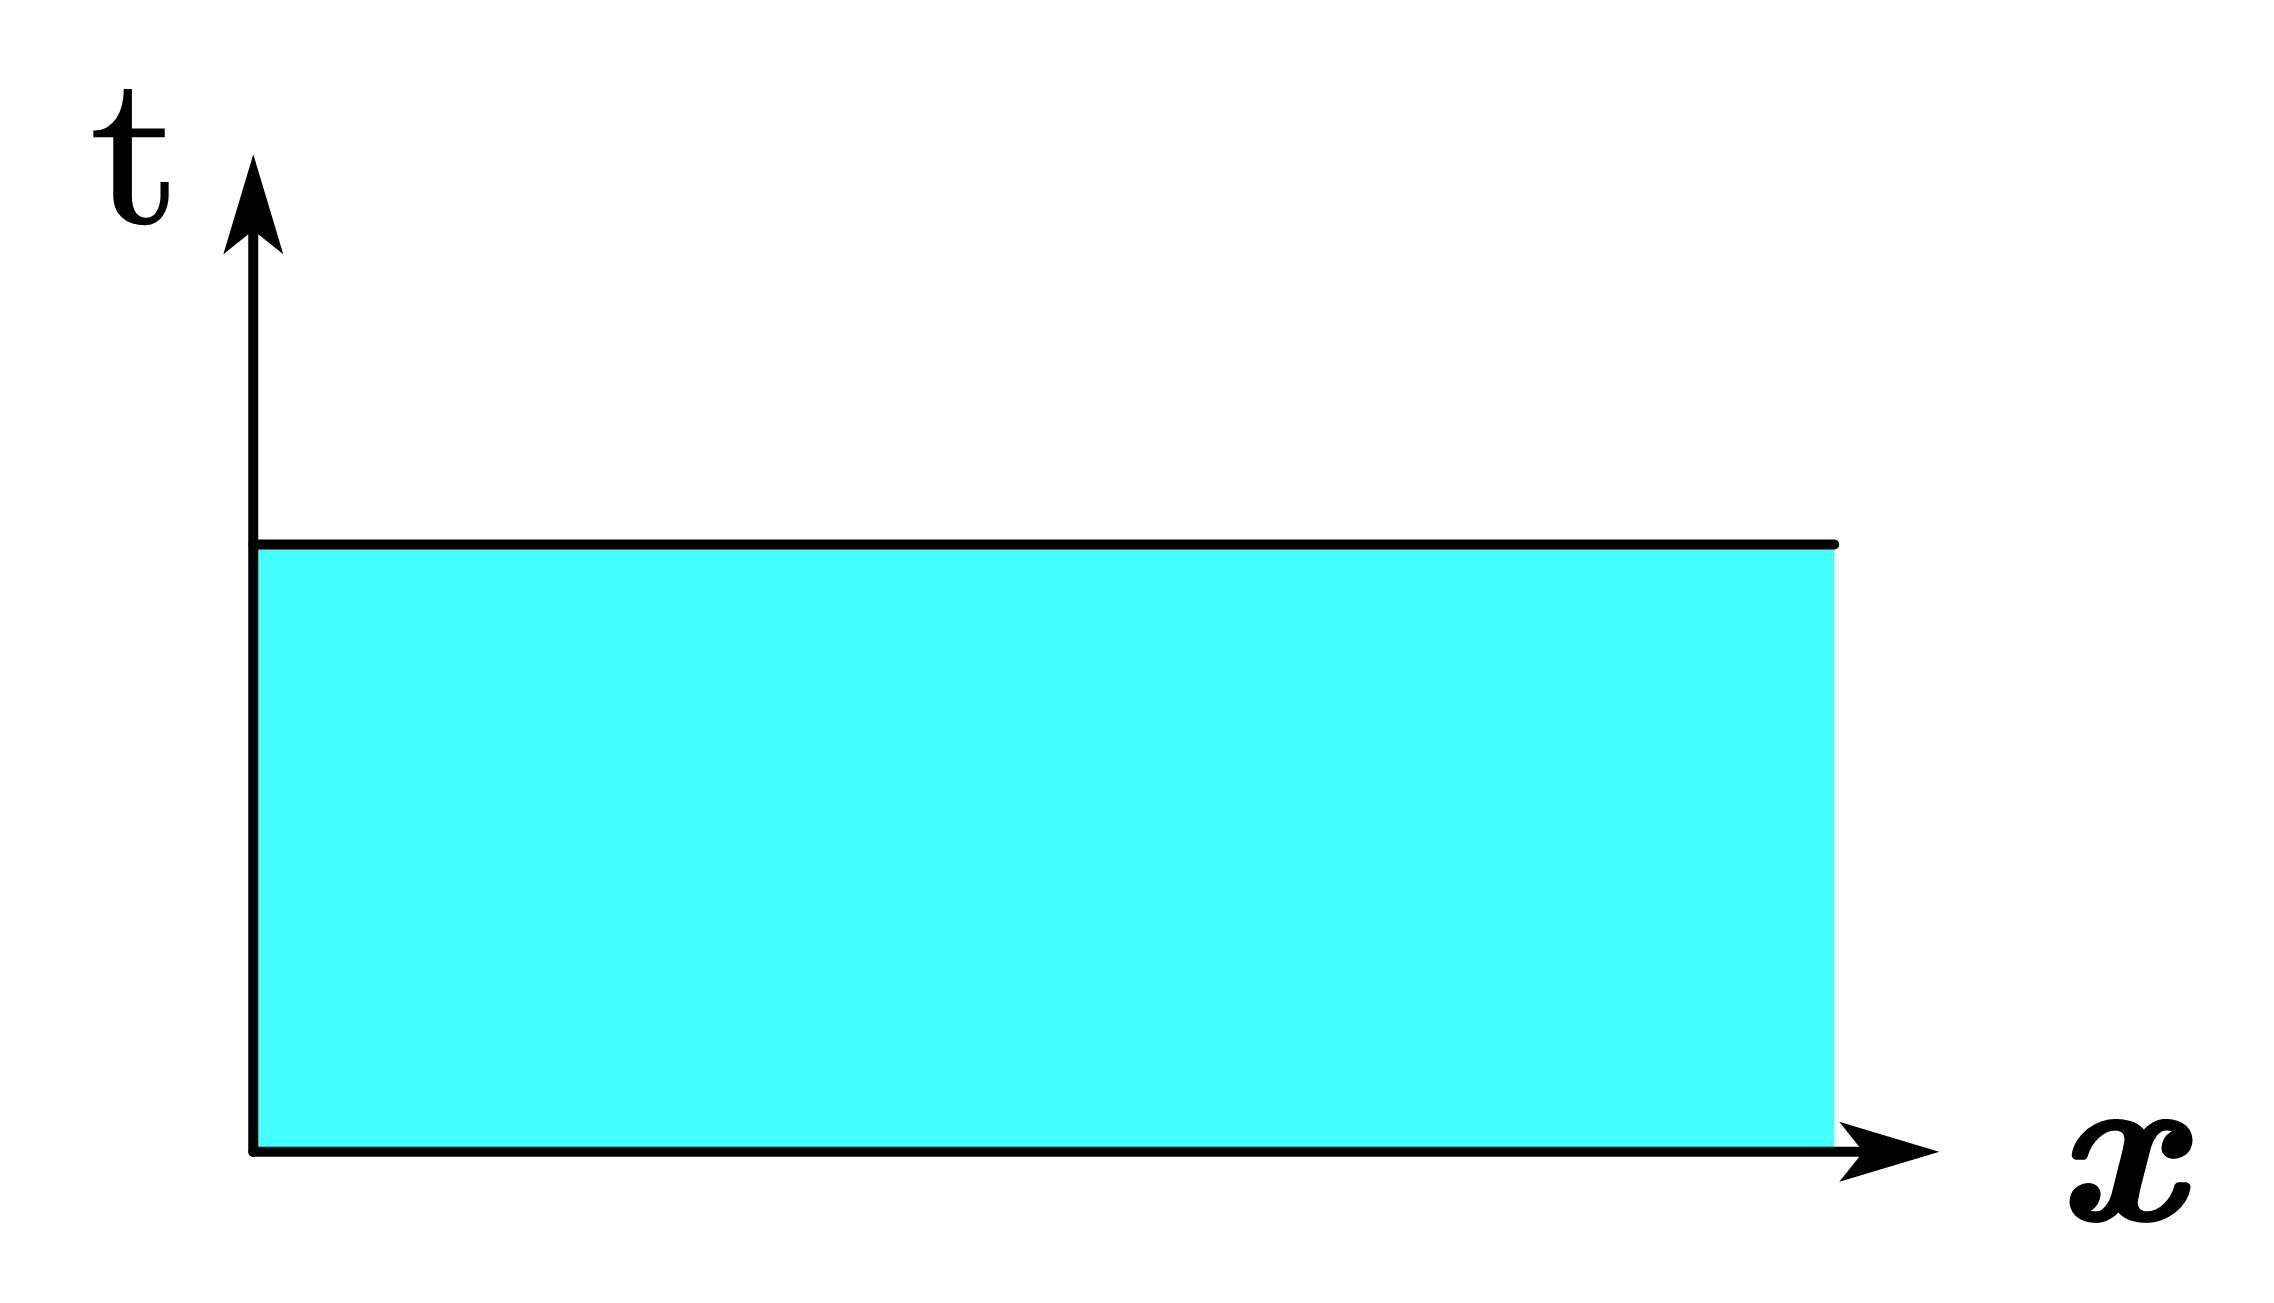
\includegraphics[width=0.50\textwidth]{half-line heat eqn.pic.jpg}
    \caption{The Heat Equation on the Half-Line}
    \label{1}
\end{figure}
\begin{subequations}\label{1.1}
    \begin{align}
        \begin{split}\label{1.1a}
        \dfrac{\partial u}{\partial t}-\dfrac{\partial^2 u}{\partial x^2}=0,\quad &0<t<T,\quad 0<x<\infty ;
        \end{split}\\[1.5mm]
        \begin{split}\label{1.1b}
        u(x,0)=f(x),\quad &0<x<\infty;
        \end{split}\\
        \begin{split}\label{1.1c}
        -\dfrac{\partial u}{\partial x}+hu=g(t),\quad &0<t<T,\quad x=0;
        \end{split}\\
        \begin{split}\label{1.1d}
        u(x,t)\to 0,\quad &0<t<T,\quad x\to\infty
        \end{split}
    \end{align}
where $h\geqslant 0$, $g\in C^1([0,T])$, $f\in L^1{(\mathbb{R}^+)}\cap C^0{(\mathbb{R}^+)}$.
\end{subequations}
\subsection{Step 1\textemdash Derive the Global Relation}
\noindent Take Eq.\eqref{1.1a} and apply the Half-Fourier Transform on both sides
\begingroup
\allowdisplaybreaks
\begin{align*}
    &\dfrac{\partial \hat{u}}{\partial t}(\lambda,t)=\int_{0}^{\infty} \dfrac{\partial u}{\partial t}{e^{-i\lambda x}}dx=\int_{0}^{\infty}\dfrac{\partial^2 u}{\partial x^2} e^{-i\lambda x}dx\\
    &=-\dfrac{\partial u}{\partial x}(0,t)+i\lambda\int_{0}^{\infty} \dfrac{\partial u}{\partial x} e^{-i\lambda x} dx\\
    &=-\dfrac{\partial u}{\partial x}(0,t)-i\lambda u(0,t)-\lambda^2\int_{0}^{\infty} u(x,t)e^{-i\lambda x}dx\\
    &=-\dfrac{\partial u}{\partial x}(0,t)-i\lambda u(0,t)-\lambda^2\hat{u}(\lambda,t).
\end{align*}
Hence, We obtained a first-order ODE
\begin{equation}\label{1.2}
    \dfrac{\partial \hat{u}}{\partial t}(\lambda,t)+\lambda^2\hat{u}(\lambda,t)=-g_1(t)-i\lambda g_0(t),\quad \text{Im}(\lambda)\leqslant 0.
\end{equation}
where $g_0(t)=u(0,t)$, $g_1(t)=u_x(x,t)\vert_{x=0}$. The solution to Eq.\eqref{1.2} is
\begin{equation}\label{1.3}
    \hat{u}(\lambda,t)=e^{-\lambda^2 t}\left(\hat{f}(\lambda)-\tilde{g_1}(\lambda^2,t)-i\lambda\tilde{g_0}(\lambda^2,t)\right),\quad \text{Im}(\lambda)\leqslant 0.
\end{equation}
where \begin{equation*}
    \tilde{g_0}(\lambda,t)=\int_{0}^{t} e^{\lambda \tau}g_0(\tau)d\tau, \quad \tilde{g_1}(\lambda,t)=\int_{0}^{t} e^{\lambda \tau}g_1(\tau)d\tau,
\end{equation*}
and $$\hat{f}(\lambda)=\int_{0}^{\infty} f(x)e^{-i\lambda x}dx.$$
Note that $\tilde{g_0}(\lambda,t)$, and $\tilde{g_1}(\lambda,t)$ are entire functions with respect to $\lambda\in\mathbb{C}$. $\hat{u}(\lambda,t)$, $\hat{f}(\lambda)$ are well-defined within $\{\lambda\in\mathbb{C}:\text{Im}(\lambda)\leqslant 0\}$. Hence, Eq.\eqref{1.3} extends to $\{\lambda\in\mathbb{C}:\text{Im}(\lambda)\leqslant 0\}$, which is the desired Global Relation. This statement can be interpreted as implying that $\hat{u}(\lambda,t)$ extends to become a holomorphic function in the lower-half $\lambda$ plane. \vspace{5mm}
\begin{figure}[h]
    \centering \hspace{5mm}
    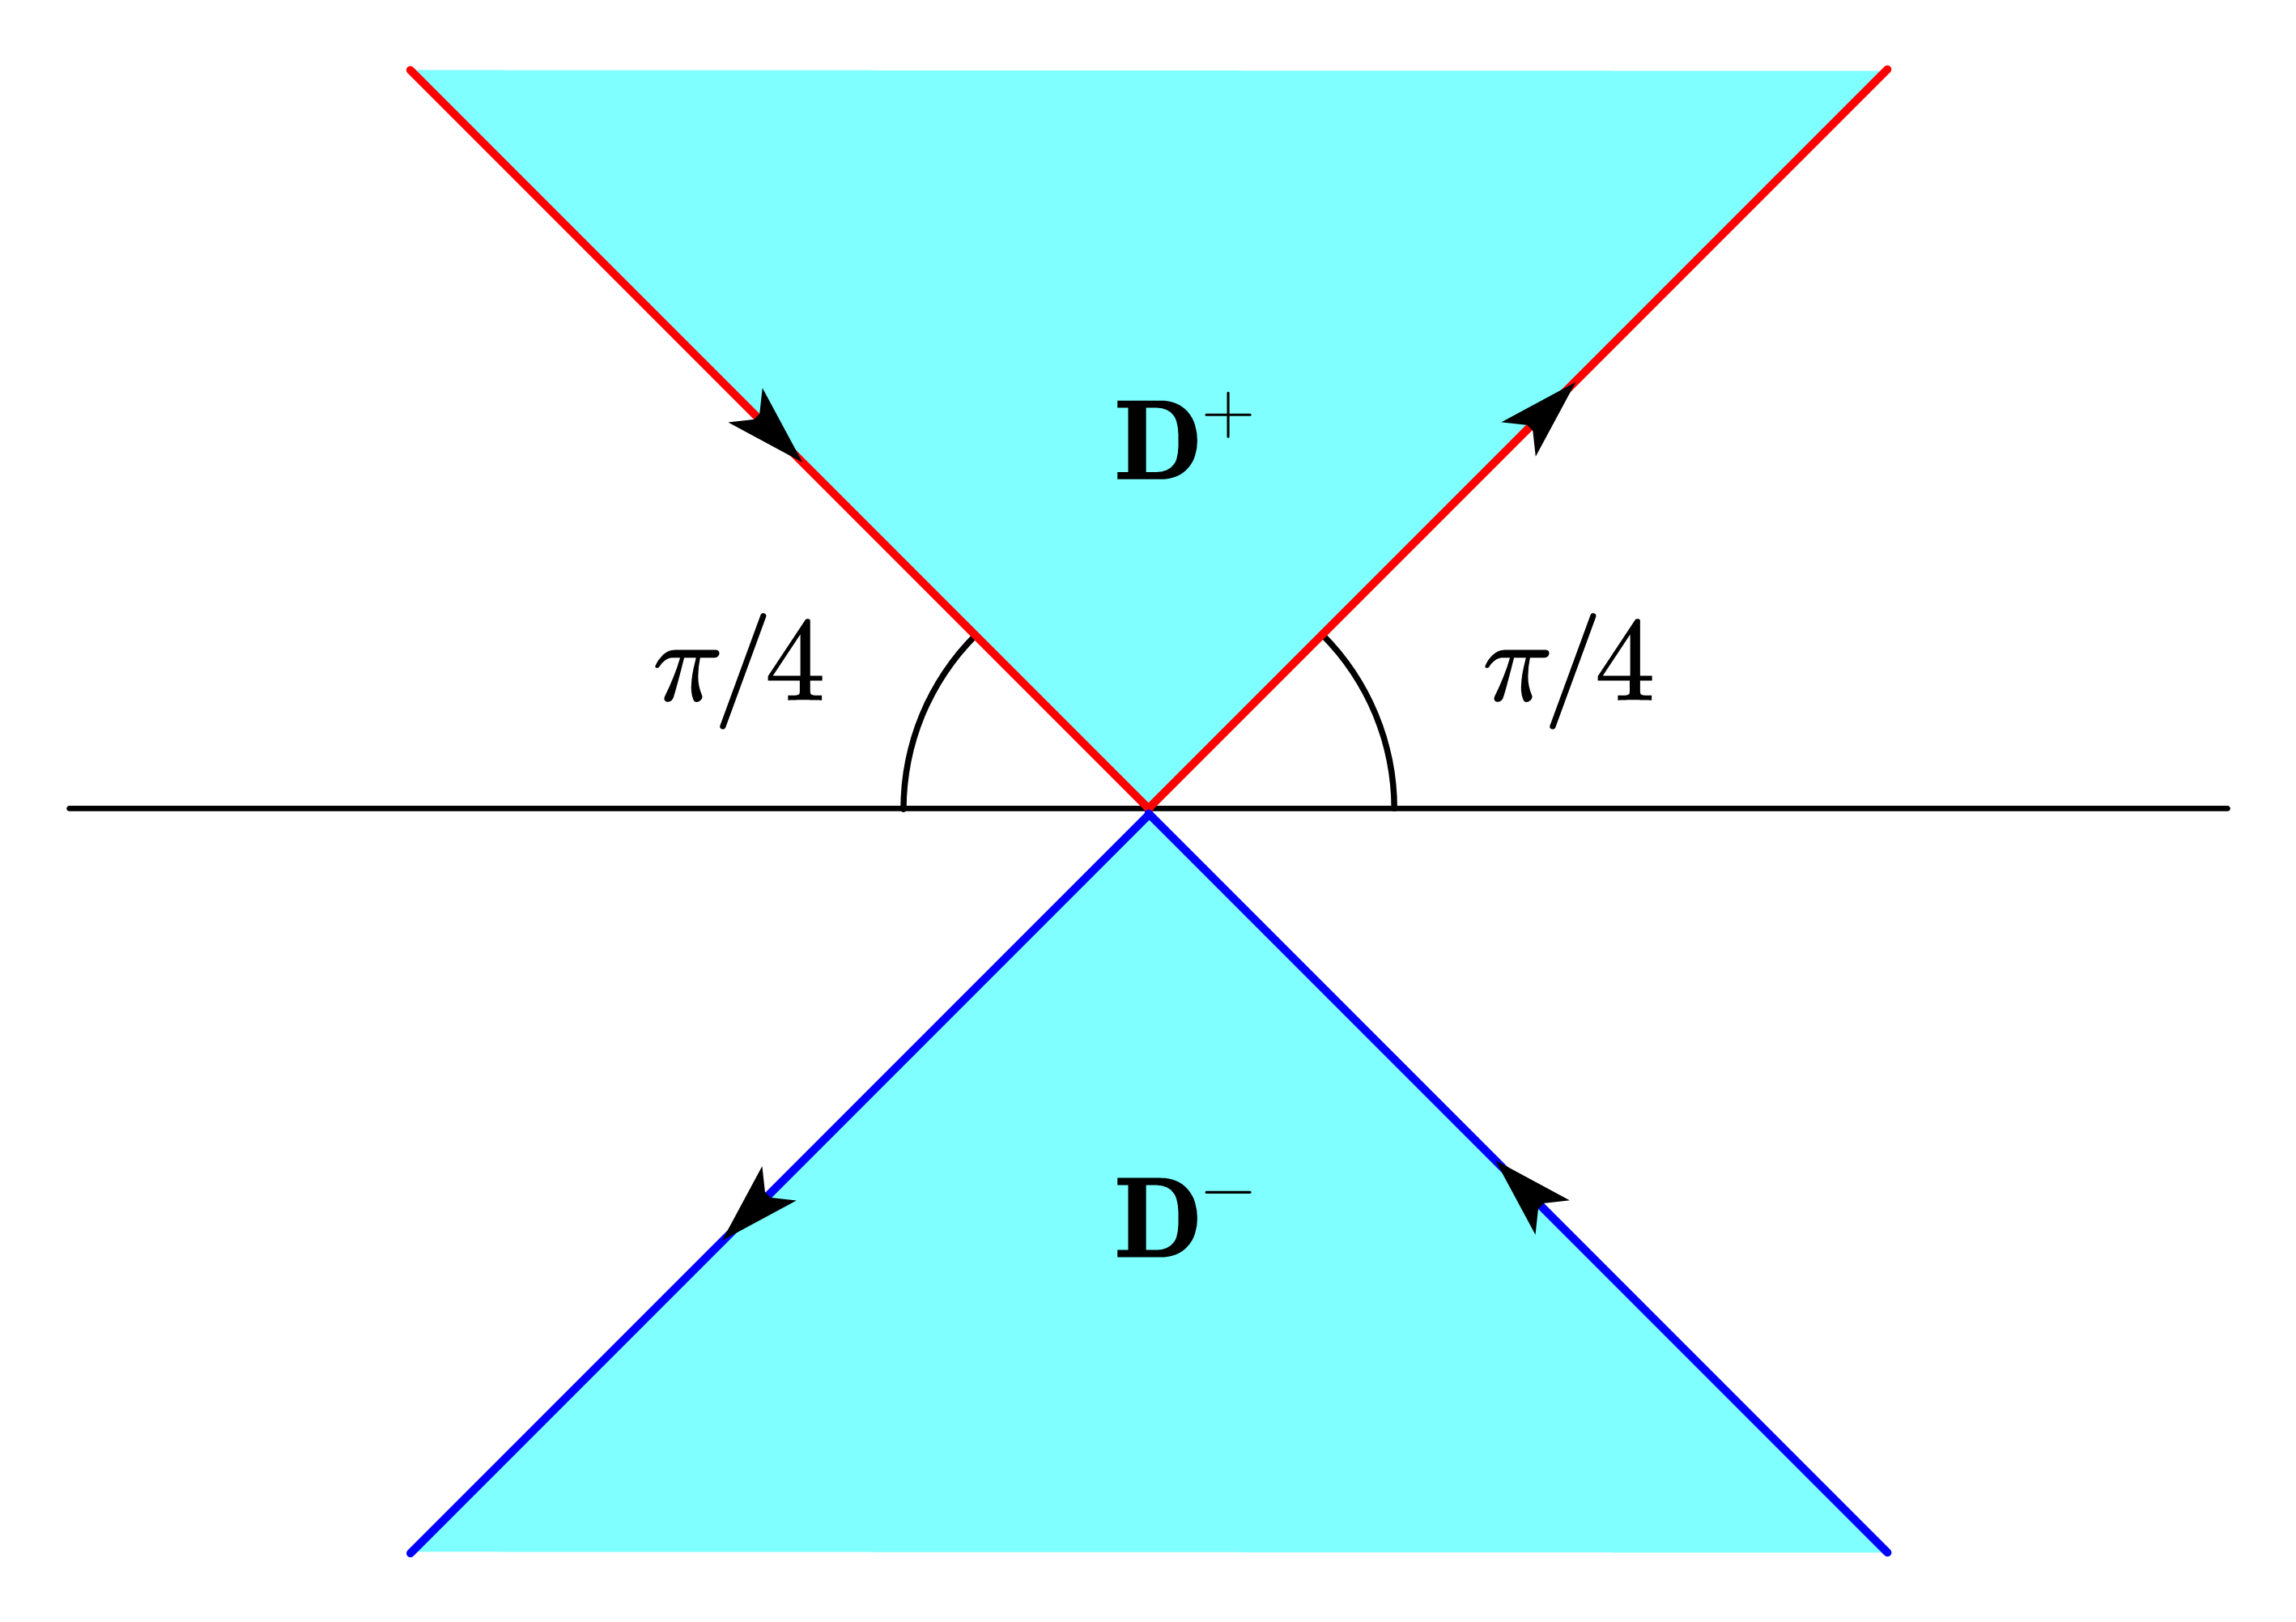
\includegraphics[width=0.60\textwidth]{D^+.pic.jpg}
    \caption{The regions $D^+$ and $D^-$ in the complex $\lambda$ plane, with $D=D^+\cup D^-$. The boundaries $\partial D^+$ and $\partial D^-$ are both equipped with counterclockwise orientation.}
    \label{2}
\end{figure}
\subsection{Step 2\textemdash Shift the Contour of Integration}
Consider the Fourier Inverse Transform of Eq.\eqref{1.3}
\begin{equation}\label{1.4}
    \begin{split}
    u(x,t)&=\dfrac{1}{2\pi}\int_{\mathbb{R}}e^{i\lambda x-\lambda^2 t}\hat{f}(\lambda)d\lambda\\
    &-\dfrac{1}{2\pi}\int_{\mathbb{R}}e^{i\lambda x-\lambda^2 t}[\tilde{g_1}(\lambda^2,t)+i\lambda \tilde{g_0}(\lambda^2,t)]d\lambda.
    \end{split}
\end{equation}
We claim Eq.\eqref{1.4} is equivalent to
\begin{equation}\label{1.5}
    \begin{split}
    u(x,t)&=\dfrac{1}{2\pi}\int_{\mathbb{R}}e^{i\lambda x-\lambda^2 t}\hat{f}(\lambda)d\lambda\\
    &-\dfrac{1}{2\pi}\int_{\partial D^+}e^{i\lambda x-\lambda^2 t}[\tilde{g_1}(\lambda^2,t)+i\lambda \tilde{g_0}(\lambda^2,t)]d\lambda.
    \end{split}
\end{equation}
where $\partial D^+$ is specified in (Fig.\ref{2}). In order to deform the contour of integration from the real line to $\partial D^+$, we use the Cauchy's Theorem and Jordan's Lemma. Consider the integrands
\begin{align}
    \begin{split}\label{1.6}
    &e^{i\lambda x-\lambda^2 t}\tilde{g_1}(\lambda^2,t)=e^{i\lambda x}\int_{0}^{t} e^{-\lambda^2(t-\tau)}g_1(\tau)d\tau
    \end{split}\\
    \begin{split}\label{1.7}
    &i\lambda e^{i\lambda x-\lambda^2 t}\tilde{g_0}(\lambda^2,t)=i\lambda e^{i\lambda x}\int_{0}^{t} e^{-\lambda^2(t-\tau)}g_0(\tau)d\tau.
    \end{split}
\end{align}
$D^+=\{\lambda\in\mathbb{C}:\text{Im}(\lambda)\geqslant 0, \text{Re}(\lambda^2)<0\}$ (See Fig.\ref{3}). On $\{\lambda\in\mathbb{C}:\text{Im}(\lambda)\geqslant 0\}-D^+$,\\ [1mm] $\vert e^{i\lambda x}\vert \leqslant 1$, because $x\geqslant 0$; and $\vert e^{-\lambda^2(t-\tau)}\vert \leqslant 1$, since $t-\tau\geqslant 0$. Apply integration by parts to Eq.\eqref{1.6}
\begin{equation*}
    e^{i\lambda x-\lambda^2 t}\tilde{g_1}(\lambda^2,t)=\dfrac{e^{i\lambda x}}{\lambda^2}\left(g_1(t)-e^{-\lambda^2 t}g_1(0)-\int_{0}^{t}e^{-\lambda^2(t-\tau)}g^{\prime}_1(\tau)d\tau\right).
\end{equation*}
Hence, $e^{-\lambda^2 t}\tilde{g_1}(\lambda^2,t)=O\left(\dfrac{1}{\lambda^2}\right)$ as $\lambda\to\infty$ in $\{\lambda\in\mathbb{C}:\text{Im}(\lambda)\geqslant 0\}-D^+$. Similarly, for Eq.\eqref{1.7},
\begin{equation*}
    i\lambda e^{i\lambda x-\lambda^2 t}\tilde{g_0}(\lambda^2,t)=\dfrac{ie^{i\lambda x}}{\lambda}\left(g_0(t)-e^{-\lambda^2 t}g_0(0)-\int_{0}^{t}e^{-\lambda^2(t-\tau)}g^{\prime}_0(\tau)d\tau\right).
\end{equation*}
Then, $ie^{-\lambda^2 t}\tilde{g_0}(\lambda^2,t)=O\left(\dfrac{1}{\lambda}\right)$ as $\lambda\to\infty$ in $\{\lambda\in\mathbb{C}:\text{Im}(\lambda)\geqslant 0\}-D^+$.
\begin{figure}[h]
    \centering \hspace{5mm}
    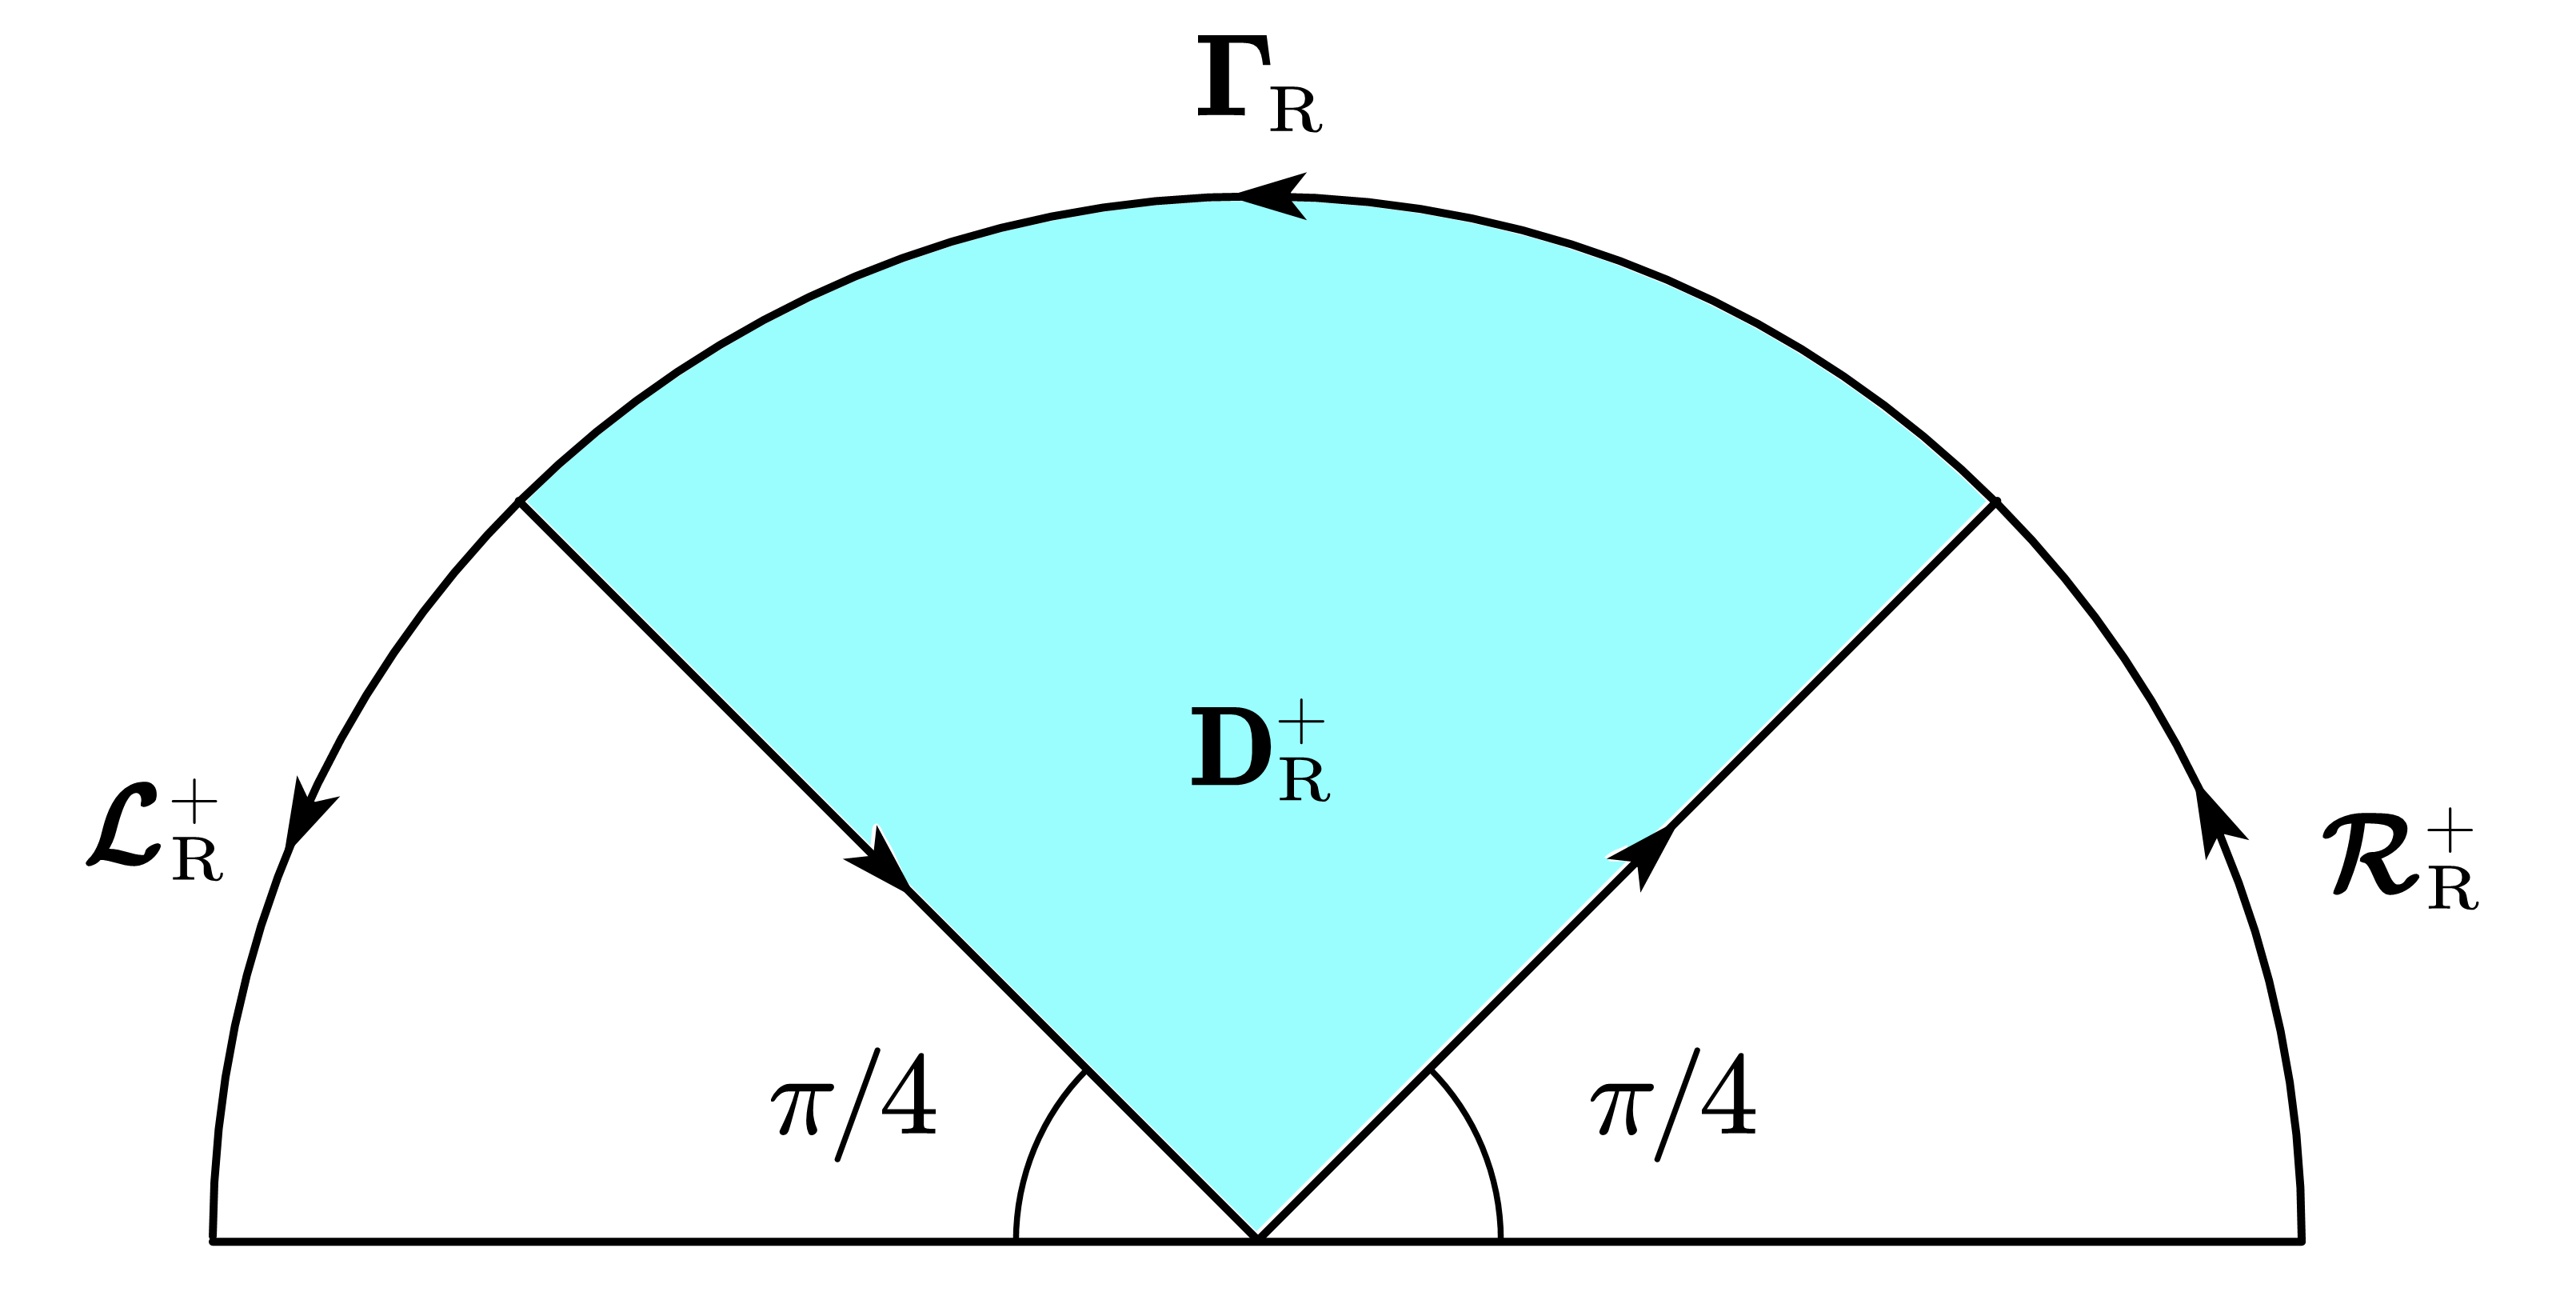
\includegraphics[width=0.60\textwidth]{344821711499232_.pic_hd.jpg}
    \caption{The contours $\mathcal{L}^{+}(R)$ and $\mathcal{R}^{+}(R)$}
    \label{3}
\end{figure}\\
By \href{https://w.wiki/9aSw}{Jordan's Lemma}, for any $x>0$:
\begin{align*}
    &\lim\limits_{R\to\infty} \int_{\mathcal{L}^+_{R}} e^{-\lambda^2 t}[\tilde{g_1}(\lambda^2,t)+i\lambda\tilde{g_0}(\lambda^2,t)]e^{i\lambda x}d\lambda=0;\\
    &\lim\limits_{R\to\infty} \int_{\mathcal{R}^+_{R}} e^{-\lambda^2 t}[\tilde{g_1}(\lambda^2,t)+i\lambda\tilde{g_0}(\lambda^2,t)]e^{i\lambda x}d\lambda=0.
\end{align*}
Apply \href{https://w.wiki/9aTM}{Cauchy's Theorem} to obtain
\begin{align*}
    &\int_{\mathbb{R}}e^{i\lambda x-\lambda^2 t}[\tilde{g_1}(\lambda^2,t)+i\lambda \tilde{g_0}(\lambda^2,t)]d\lambda\\
    =&\int_{\partial D^+}e^{i\lambda x-\lambda^2 t}[\tilde{g_1}(\lambda^2,t)+i\lambda \tilde{g_0}(\lambda^2,t)]d\lambda.
\end{align*}
Therefore, Eq.\eqref{1.5} holds. But it is not a solution of the \href{https://w.wiki/9aTe}{Ehrenpreis form}, namely of the form
\begin{equation}\label{1.8}
    u(x,t)=\int U(\lambda)e^{i\lambda x-\lambda^2 t} d\lambda.
\end{equation}
Moreover, $\tilde{g_0}(\lambda^2,t)$ and $\tilde{g_1}(\lambda^2,t)$ remain unsolved.
\subsection{Step 3\textemdash Eliminate the Unknowns}
To complete our solution, we need to use the boundary conditions and the Global Relation to solve for $\tilde{g_0}$ and $\tilde{g_1}$.  Multiply $e^{\lambda^2\tau}$ on both sides of \eqref{1.1c} and integrate with respect to $\tau$:
\begin{equation}\label{1.9}
    -\tilde{g_1}(\lambda^2,t)+h\tilde{g_0}(\lambda^2,t)=\int_{0}^{t} e^{\lambda^2\tau}g(\tau)d\tau=\tilde{g}(\lambda^2,t).
\end{equation}
Eq.\eqref{1.9} provides us with one equation to solve for $\tilde{g_0}(\lambda^2,t)$ and $\tilde{g_1}(\lambda^2,t)$, we need another equation. It turns out a clever manipulation of the Global Relation\eqref{1.3} offers the equation we need.

Note that Eq.\eqref{1.3} is valid in the lower-half complex $\lambda$ plane, but the range of integration of Eq.\eqref{1.5} is located in the upper-half plane. It is natural to consider replacing $\lambda$ by $-\lambda$, noticing that this substitution does affect $\tilde{g_0}(\lambda^2,t)$ and $\tilde{g_1}(\lambda^2,t)$:
\begin{equation}\label{1.10}
    \hat{u}(-\lambda,t)e^{\lambda^2 t}=\hat{f}(-\lambda)-\tilde{g_1}(\lambda^2,t)+i\lambda\tilde{g_0}(\lambda^2,t), \quad \text{Im}(\lambda)\geqslant 0.
\end{equation}
Combine Eq.\eqref{1.9} and Eq.\eqref{1.10} to obtain the matrix equation
\begin{align*}
    &\mathbb{A}\boldsymbol{v}=\boldsymbol{b}, \quad \text{where} \quad
    \mathbb{A}= \begin{pmatrix} h & -1\\ -i\lambda & 1 \end{pmatrix},\\
    &\boldsymbol{v}= \begin{pmatrix} \tilde{g_0}(\lambda^2,t) \\ \tilde{g_1}(\lambda^2,t) \end{pmatrix}, \quad \text{and} \quad 
    \boldsymbol{b}=\begin{pmatrix} \tilde{g}(\lambda^2,t) \\ \hat{f}(-\lambda)-\hat{u}(-\lambda,t)e^{\lambda^2 t} \end{pmatrix}.
\end{align*}
Then the solution for $\boldsymbol{v}$ is
\begin{equation*}
    \begin{split}
    \boldsymbol{v}&=\mathbb{A}^{-1}b=\dfrac{1}{h-i\lambda}\begin{pmatrix} 1 & 1 \\ i\lambda & h \end{pmatrix} \begin{pmatrix} \tilde{g}(\lambda^2,t) \\ \hat{f}(-\lambda)-\hat{u}(-\lambda,t)e^{\lambda^2 t} \end{pmatrix}\\
    &=\dfrac{1}{h-i\lambda} \begin{pmatrix} \tilde{g}(\lambda^2,t)+\hat{f}(-\lambda)-\hat{u}(-\lambda,t)e^{\lambda^2 t}\\ i\lambda \tilde{g}(\lambda^2,t)+h\hat{f}(-\lambda)-h\hat{u}(-\lambda,t)e^{\lambda^2 t} \end{pmatrix}.
    \end{split}
\end{equation*}
Thus,\begin{equation}\label{1.11}
    \begin{split}
    &\tilde{g_1}(\lambda^2,t)+i\lambda\tilde{g_0}(\lambda^2,t)=\langle (i\lambda,1),\boldsymbol{v}\rangle\\
    &=\dfrac{1}{h-i\lambda}\left(2i\lambda\tilde{g}(\lambda^2,t)+(h+i\lambda)[\hat{f}(-\lambda)-\hat{u}(-\lambda,t)e^{\lambda^2 t}]\right),
    \end{split}
\end{equation}
which can be inserted into Eq.\eqref{1.5} to obtain:
\begin{equation}\label{1.12}
    \begin{split}
        &u(x,t)=\dfrac{1}{2\pi}\int_{\mathbb{R}}e^{i\lambda x-\lambda^2 t}\hat{f}(\lambda)d\lambda\\
        &-\dfrac{1}{2\pi} \int_{\partial D^+} \dfrac{e^{i\lambda x-\lambda^2 t}}{h-i\lambda}\left(2i\lambda\tilde{g}(\lambda^2,t)+(h+i\lambda)[\hat{f}(-\lambda)-\hat{u}(-\lambda,t)e^{\lambda^2 t}]\right) d\lambda.
    \end{split}
\end{equation}\label{SSec 1.3}
But we are not done with such an expression, since $\hat{u}(-\lambda,t)$ is an unknown. The situation seems a bit frustrating, because we have run out of equations. 
Fortunately, it turns out that the contribution of $\hat{u}(-\lambda,t)$ vanishes. This is again due to \href{https://w.wiki/9aTM}{Cauchy's Theorem}.
The term $\hat{u}(-\lambda,t)$ gives rise to a contribution of 
\begin{equation*}
    \dfrac{1}{2\pi}\int_{\partial D^+}\dfrac{h+i\lambda}{h-i\lambda}\hat{u}(-\lambda,t)e^{i\lambda x}d\lambda,
\end{equation*}
where $\hat{u}(-\lambda,t)$ is bounded in the upper-half $\lambda$ plane. In fact,
\begin{equation*}
    \begin{split}
      &\vert\hat{u}(-\lambda,t)\vert=\left|\int_{0}^{\infty} u(x,t)e^{i\lambda x} dx\right|=\int_{0}^{\infty} \vert u(x,t)e^{-\text{Im}(\lambda)x}\vert dx<\infty,\quad \text{Im}(\lambda)> 0.
    \end{split}
\end{equation*}
Since $\lim\limits_{x\to\infty} u(x,t)=0\Rightarrow u(x,t)e^{-\text{Im}(\lambda)x}\sim o(e^{-\text{Im}(\lambda)x})$, as $x\to\infty$.
Let's denote $D^+\cap\{\lambda\in\mathbb{C}:\vert\lambda\vert=R\}$ as $\Gamma_{R}$ (See Fig.[\ref{3}]), then 
\begin{equation*}
    \left|\dfrac{h+i\lambda}{h-i\lambda}\right|\leqslant \dfrac{R+h}{R-h}\leqslant 3, \quad \lambda\in\Gamma_{R},\quad R\geqslant 2h.
\end{equation*}
For all $x>0$:
\begin{align*}
    &\left| \int_{\Gamma_R} \dfrac{h+i\lambda}{h-i\lambda}\hat{u}(-\lambda,t)e^{i\lambda x}d\lambda\right|\lesssim R\int_{\pi/4}^{3\pi/4} e^{-xR\sin\theta} d\theta=2R\int_{\pi/4}^{\pi/2}e^{-xR\sin\theta}d\theta\\
    &\leqslant 2R\int_{\pi/4}^{\pi/2} e^{-{2xR\theta}/{\pi}} d\theta=\dfrac{\pi}{x}\left(e^{-{xR}/{2}}-e^{-{xR}/{4}}\right)\longrightarrow 0, \quad \text{as}\quad  R \to\infty.
\end{align*}
Note that if $h=0$, $\lambda=0$ would be a removable singularity of $\dfrac{h+i\lambda}{h-i\lambda}$. Thus, $\dfrac{h+i\lambda}{h-i\lambda}\hat{u}(-\lambda,t)e^{i\lambda x}$ is holomorphic in $\{\lambda\in\mathbb{C}: \text{Im}(\lambda)\geqslant 0\}$ . By \href{https://w.wiki/9aTM}{Cauchy's Theorem},
\begin{equation}\label{1.13}
    \int_{\partial D^+}\dfrac{h+i\lambda}{h-i\lambda}\hat{u}(-\lambda,t)e^{i\lambda x}d\lambda=-\lim\limits_{R\to\infty} \int_{\Gamma_R} \dfrac{h+i\lambda}{h-i\lambda}\hat{u}(-\lambda,t)e^{i\lambda x}d\lambda=0.
\end{equation}
Insert Eq.\eqref{1.13} into Eq.\eqref{1.14} to acquire
\begin{equation}\label{1.14}
    \begin{split}
        u(x,t)&=\dfrac{1}{2\pi}\int_{\mathbb{R}}e^{i\lambda x-\lambda^2 t}\hat{f}(\lambda)d\lambda\\
        &-\dfrac{1}{2\pi} \int_{\partial D^+} e^{i\lambda x-\lambda^2 t}\left(\dfrac{2i\lambda}{h-i\lambda}\tilde{g}(\lambda^2,t)+\dfrac{h+i\lambda}{h-i\lambda}\hat{f}(-\lambda)\right) d\lambda.
    \end{split}
\end{equation}
However, Eq.\eqref{1.14} is still not of the form of Eq.\eqref{1.8}. We can refine our solution by tackling with the boundary conditions even more.
\subsection{Refine the Solution to the Ehrenpreis Form}\label{SSec 1.4}
By Eq.\eqref{1.1c}, the heat equation is valid for $0<t<T$. Let
\begin{equation}\label{1.15}
    \begin{split}
    &\tilde{g_0}(\lambda)=\tilde{g_0}(\lambda,T)=\int_{0}^{T} e^{\lambda \tau}g_{0}(\tau) d\tau;\\
    &\tilde{g_1}(\lambda)=\tilde{g_1}(\lambda,T)=\int_{0}^{T} e^{\lambda \tau}g_{0}(\tau) d\tau;\\
    &\tilde{g}(\lambda)=\tilde{g}(\lambda,T)=\int_{0}^{T} e^{\lambda \tau} g(\tau) d\tau.
    \end{split}
\end{equation}
Then, Eq.\eqref{1.5} is equivalent to the equation
\begin{equation}\label{1.16}
    \begin{split}
        u(x,t)&=\dfrac{1}{2\pi}\int_{\mathbb{R}}e^{i\lambda x-\lambda^2 t}\hat{f}(\lambda)d\lambda\\
        &-\dfrac{1}{2\pi}\int_{\partial D^+}e^{i\lambda x-\lambda^2 t}[\tilde{g_1}(\lambda^2)+i\lambda \tilde{g_0}(\lambda^2)]d\lambda.
    \end{split}
\end{equation}
Although Eq.\eqref{1.5} and Eq.\eqref{1.16} differ by
\begin{equation}\label{1.17}
    \dfrac{1}{2\pi}\int_{\partial D^+} e^{i\lambda x}\left[ \int_{t}^{T} \left(e^{-\lambda^2(t-\tau)}g_1(\tau)+i\lambda e^{-\lambda^2(t-\tau)}g_0(\tau)\right)d\tau \right]d\lambda.
\end{equation}
Again, integration by parts, \href{https://w.wiki/9aTM}{Cauchy's Theorem} supplemented with \href{https://w.wiki/9aSw}{Jordan's Lemma} imply that Eq.\eqref{1.17} vanishes. Note that $\tau\geqslant t$ in Eq.\eqref{1.17} and $\text{Re}(\lambda^2)<0$ in $D^+$ are crucial here, as we deform the contour of integration from $\partial D^+$ to $\Gamma_{R}$.

Analogously, Eq.\eqref{1.14} is equivalent to the equation
\begin{equation}\label{1.18}
    \begin{split}
        u(x,t)&=\dfrac{1}{2\pi}\int_{\mathbb{R}}e^{i\lambda x-\lambda^2 t}\hat{f}(\lambda)d\lambda\\
        &-\dfrac{1}{2\pi} \int_{\partial D^+} e^{i\lambda x-\lambda^2 t}\left(\dfrac{2i\lambda}{h-i\lambda}\tilde{g}(\lambda^2)+\dfrac{h+i\lambda}{h-i\lambda}\hat{f}(-\lambda)\right) d\lambda.
    \end{split}
\end{equation}
In fact, Eq.\eqref{1.14} and Eq.\eqref{1.18} differ by
\begin{equation}\label{1.19}
    \dfrac{1}{2\pi}\int_{\partial D^+} \left( \dfrac{2i\lambda}{h-i\lambda}\int_{t}^{T} e^{-\lambda^2(t-\tau)}g(\tau)d\tau \right)e^{i\lambda x}d\lambda.
\end{equation}
Note that \begin{equation*}
    \begin{split}
    &\left|\dfrac{2i\lambda}{h-i\lambda}\right|\leqslant \dfrac{2R}{R-h}\leqslant 4,\quad\lambda\in\Gamma_{R},\quad R\geqslant 2h;\\
    &\left|\int_{t}^{T} e^{-\lambda^2(t-\tau)}g(\tau)d\tau\right|\leqslant \int_{0}^{T} \vert g(\tau)\vert d\tau<\infty.
    \end{split}
\end{equation*}
Similar to the estimate made in the previous subsection, we have
\begin{equation*}
    \lim\limits_{R\to \infty}\int_{\Gamma_R} \left( \dfrac{2i\lambda}{h-i\lambda}\int_{t}^{T} e^{-\lambda^2(t-\tau)}g(\tau)d\tau \right)e^{i\lambda x}d\lambda=0.
\end{equation*}
It follows from \href{https://w.wiki/9aTM}{Cauchy's Theorem} that Eq.\eqref{1.18} vanishes. Hence, we obtain a solution of the \href{https://w.wiki/9aTe}{Ehrenpreis form}, which is given by Eq.\eqref{1.18}.
It remains to verify that Eq.\eqref{1.18} is the solution to Eq.\eqref{1.1}.
\subsection{Verify the Solution}
Consider Eq.\eqref{1.18}, the $(x,t)$ dependence lies only within the term $e^{i\lambda x-\lambda^2 t}$, which clearly satisfies the heat equation. It is intuitively obvious that Eq.\eqref{1.18} should satisfy the heat equation. Let's verify that.
\begin{equation}\label{1.20}
    \int_{\mathbb{R}} \dfrac{\partial}{\partial t} e^{i\lambda x-\lambda^2 t} \hat{f(\lambda)}d\lambda=-\int_{\mathbb{R}} \lambda^2 e^{i\lambda x-\lambda^2 t}\hat{f}(\lambda)d\lambda.
\end{equation}
Since $\hat{f}(\lambda)$ is bounded by $\Vert f\Vert_{L^1({\mathbb{R^+}})}$, $\lambda^2e^{i\lambda x-\lambda^2 t}\in L^1(\mathbb{R})$, it follows from the \href{https://w.wiki/9asL}{Dominated Convergence Theorem} that
\begin{equation}\label{1.21}
    \dfrac{\partial}{\partial t} \int_{\mathbb{R}}e^{i\lambda x-\lambda^2 t} \hat{f(\lambda)}d\lambda=\int_{\mathbb{R}} \dfrac{\partial}{\partial t} e^{i\lambda x-\lambda^2 t} \hat{f(\lambda)}d\lambda.
\end{equation}
Combine Eq.\eqref{1.20} and Eq.\eqref{1.21} to write
\begin{equation}\label{1.22}
    \dfrac{\partial}{\partial t} \int_{\mathbb{R}}e^{i\lambda x-\lambda^2 t} \hat{f(\lambda)}d\lambda=-\int_{\mathbb{R}} \lambda^2 e^{i\lambda x-\lambda^2 t}\hat{f}(\lambda)d\lambda.
\end{equation}
Similary, we have the the $x$ derivative
\begin{equation}\label{1.23}
    \dfrac{\partial^2}{\partial x^2} \int_{\mathbb{R}}e^{i\lambda x-\lambda^2 t} \hat{f(\lambda)}d\lambda=-\int_{\mathbb{R}} \lambda^2 e^{i\lambda x-\lambda^2 t}\hat{f}(\lambda)d\lambda.
\end{equation}
Join Eq.\eqref{1.22} and Eq.\eqref{1.23} to obtained
\begin{equation}\label{1.24}
    \left(\dfrac{\partial}{\partial t}-\dfrac{\partial^2}{\partial x^2}\right)\int_{\mathbb{R}}e^{i\lambda x-\lambda^2 t} \hat{f(\lambda)}d\lambda=0.
\end{equation}
Analogously, It is easy to verify that 
\begin{equation}\label{1.25}
    \begin{split}
    &\left(\dfrac{\partial}{\partial t}-\dfrac{\partial^2}{\partial x^2}\right)\int_{\partial D^+} e^{i\lambda x-\lambda^2 t}\left(\dfrac{2i\lambda}{h-i\lambda}\tilde{g}(\lambda^2)+\dfrac{h+i\lambda}{h-i\lambda}\hat{f}(-\lambda)\right) d\lambda\\
    =&\int_{\partial D^+} \left(\dfrac{\partial}{\partial t}-\dfrac{\partial^2}{\partial x^2}\right)e^{i\lambda x-\lambda^2 t}\left(\dfrac{2i\lambda}{h-i\lambda}\tilde{g}(\lambda^2)+\dfrac{h+i\lambda}{h-i\lambda}\hat{f}(-\lambda)\right) d\lambda=0.
    \end{split}
\end{equation}
Eq.\eqref{1.24} with Eq.\eqref{1.25} suggest that Eq.\eqref{1.18} satisfies Eq.\eqref{1.1a}. Next, we shall show that Eq.\eqref{1.18} causes no conflict with the boundary conditions Eq.\eqref{1.1b} and Eq.\eqref{1.1c}.
Evaluate Eq.\eqref{1.18} at $t=0$, $x>0$, we find
\begin{equation}\label{1.26}
    \begin{split}
        u(x,0)&=\dfrac{1}{2\pi}\int_{\mathbb{R}}e^{i\lambda x}\hat{f}(\lambda)d\lambda\\
        &-\dfrac{1}{2\pi} \int_{\partial D^+} e^{i\lambda x}\left(\dfrac{2i\lambda}{h-i\lambda}\tilde{g}(\lambda^2)+\dfrac{h+i\lambda}{h-i\lambda}\hat{f}(-\lambda)\right) d\lambda.
    \end{split}
\end{equation}
Using the boundedness of $\tilde{g}(\lambda^2)$, $\hat{f}(-\lambda)$, $\dfrac{2i\lambda}{h-i\lambda}$ and $\dfrac{h+i\lambda}{h-i\lambda}$ on $\Gamma_{R}$, Similar to the arguments made to obtain Eq.\eqref{1.13}, we have
\begin{equation}
    \begin{split}
        &\int_{\partial D^+} e^{i\lambda x}\left(\dfrac{2i\lambda}{h-i\lambda}\tilde{g}(\lambda^2)+\dfrac{h+i\lambda}{h-i\lambda}\hat{f}(-\lambda)\right) d\lambda\\
        &=-\lim\limits_{R\to\infty} \int_{\Gamma_{R}} e^{i\lambda x}\left(\dfrac{2i\lambda}{h-i\lambda}\tilde{g}(\lambda^2)+\dfrac{h+i\lambda}{h-i\lambda}\hat{f}(-\lambda)\right) d\lambda=0.
    \end{split}
\end{equation}
Thus, by the \href{https://w.wiki/9av5}{Fourier Inversion theorem}, Eq.\eqref{1.26} becomes
\begin{equation}
    u(x,0)=\dfrac{1}{2\pi}\int_{\mathbb{R}}e^{i\lambda x}\hat{f}(\lambda)d\lambda=f(x),
\end{equation}
which is Eq.\eqref{1.1b}. Note that if we drop the condition that $f\in C^{0}(\mathbb{R}^+)$, we would have $\lim\limits_{t\to 0}u(x,t)=f(x)$ almost everywhere. Now evaluate Eq.\eqref{1.18} at $x=0$, $t>0$, we find
\begin{equation}\label{1.29}
    \begin{split}
        u(0,t)&=\dfrac{1}{2\pi}\int_{\mathbb{R}}e^{-\lambda^2 t}\hat{f}(\lambda)d\lambda\\
        &-\dfrac{1}{2\pi} \int_{\partial D^+} e^{-\lambda^2 t}\left(\dfrac{2i\lambda}{h-i\lambda}\tilde{g}(\lambda^2)+\dfrac{h+i\lambda}{h-i\lambda}\hat{f}(-\lambda)\right) d\lambda.
    \end{split}
\end{equation}
Take the $x$ derivative of Eq.\eqref{1.18} and evaluate at $x=0$, $t>0$, we find
\begin{equation}\label{1.30}
    \begin{split}
        &u_x(x,t)|_{x=0}=\dfrac{1}{2\pi}\int_{\mathbb{R}}i\lambda e^{-\lambda^2 t}\hat{f}(\lambda)d\lambda\\
        &-\dfrac{1}{2\pi} \int_{\partial D^+} i\lambda e^{-\lambda^2 t}\left(\dfrac{2i\lambda}{h-i\lambda}\tilde{g}(\lambda^2)+\dfrac{h+i\lambda}{h-i\lambda}\hat{f}(-\lambda)\right) d\lambda.
    \end{split}
\end{equation}
$h$ times Eq.\eqref{1.29} and minus Eq.\eqref{1.30}, we obtain
\begin{equation}\label{1.31}
    \begin{split}
        &-u_x(x,t)|_{x=0}+hu(0,t)=\dfrac{1}{2\pi}\int_{\mathbb{R}}(h-i\lambda) e^{-\lambda^2 t}\hat{f}(\lambda)d\lambda\\
        &-\dfrac{1}{2\pi} \int_{\partial D^+} (h+i\lambda)e^{-\lambda^2 t}\hat{f}(-\lambda)d\lambda-\dfrac{1}{2\pi}\int_{\partial D^+}2i\lambda e^{-\lambda^2 t} \tilde{g}(\lambda^2)d\lambda.
    \end{split}
\end{equation}
Deform the second integral of Eq.\eqref{1.31} to the real line by \href{https://w.wiki/9aTM}{Cauchy's Theorem} and \href{https://w.wiki/9aSw}{Jordan's Lemma}:
\begin{equation}\label{1.32}
    \begin{split}
    &\dfrac{1}{2\pi}\int_{\partial D^+} (h+i\lambda) e^{-\lambda^2 t}\hat{f}(-\lambda) d\lambda\\
    =&\dfrac{1}{2\pi}\int_{\mathbb{R}} (h+i\lambda)e^{-\lambda^2 t} \hat{f}(-\lambda)d\lambda=\dfrac{1}{2\pi}\int_{\mathbb{R}} (h-i\lambda) e^{-\lambda^2 t}\hat{f}(\lambda)d\lambda.
    \end{split}
\end{equation}
Plug Eq.\eqref{1.32} into Eq.\eqref{1.31} to find Eq.\eqref{1.1c} is satisfied:
\begin{equation}\label{1.33}
    \begin{split}
        &-u_x(x,t)|_{x=0}+hu(0,t)=-\dfrac{1}{2\pi} \int_{\partial D^+} 2i\lambda e^{-\lambda^2 t}\tilde{g}(\lambda^2)d\lambda\\
        &=\dfrac{1}{2\pi} \int_{\mathbb{R}} e^{i\mu t}\tilde{g}(-i \mu)d\mu=\dfrac{1}{2\pi}\int_{\mathbb{R}}e^{i\mu t}\left(\int_{0}^{T}e^{-i\mu \tau} g(\tau)d\tau\right)d\mu\\
        &=g(t), \qquad \text{where}\quad \mu=i\lambda^2\in\mathbb{R}.
    \end{split}
\end{equation}
The last equality of Eq.\eqref{1.33} is due to the \href{https://w.wiki/9av5}{Fourier Inversion theorem}.
It remains to check that Eq.\eqref{1.18} satisfies Eq.\eqref{1.1d}. Since $\hat{f}(\lambda)$, $\tilde{g}(\lambda^2)$, $\hat{f}(-\lambda)$, $\dfrac{2i\lambda}{h-i\lambda}$ and $\dfrac{h+i\lambda}{h-i\lambda}$ are bounded$\left(\text{it is easy to verify that}\left|\dfrac{2i\lambda}{h-i\lambda}\right|\leqslant 2, \left|\dfrac{h+i\lambda}{h-i\lambda}\right|\leqslant 1, \lambda\in \partial D^+\right)$, and $e^{-\lambda^2 t}$ is simply oscillatory on $\partial D^+$. Hence,
\begin{equation*}
    \int_{\partial D^+} e^{i\lambda x-\lambda^2 t}\left(\dfrac{2i\lambda}{h-i\lambda}\tilde{g}(\lambda^2)+\dfrac{h+i\lambda}{h-i\lambda}\hat{f}(-\lambda)\right) d\lambda=O(\dfrac{1}{x}),\quad x\to\infty.
\end{equation*}
Besides, the \href{https://w.wiki/9c$f}{Riemann-Lebesgue Lemma} implies $\mathcal{F}^{-1}(L^1(\mathbb{R}))\subset C_0(\mathbb{R})$. That is to say
\begin{equation*}
    \hat{f}(\lambda)\leqslant \Vert f\Vert_{L^1(\mathbb{R^+})}\Rightarrow e^{-\lambda^2 t}\hat{f}(\lambda)\in L^1(\mathbb{R})\Rightarrow \lim\limits_{x\to\infty} \int_{\mathbb{R}}e^{i\lambda x-\lambda^2 t}\hat{f}(\lambda)d\lambda=0.
\end{equation*}
This confirms the regularity condition Eq.\eqref{1.1d}.
Therefore, the solution to Eq.\eqref{1.1} is indeed Eq.\eqref{1.18}:
\begin{equation*}
    \begin{split}
        u(x,t)&=\dfrac{1}{2\pi}\int_{\mathbb{R}}e^{i\lambda x-\lambda^2 t}\hat{f}(\lambda)d\lambda\\
        &-\dfrac{1}{2\pi} \int_{\partial D^+} e^{i\lambda x-\lambda^2 t}\left(\dfrac{2i\lambda}{h-i\lambda}\tilde{g}(\lambda^2)+\dfrac{h+i\lambda}{h-i\lambda}\hat{f}(-\lambda)\right) d\lambda.
    \end{split}
\end{equation*}
\vspace{2mm}
\subsection{The Inhomogeneous Problem}
\vspace{2mm}
Consider the inhomogeneous version of Eq.\eqref{1.1}
\begin{subequations}\label{1.34}
    \begin{align}
        \begin{split}\label{1.34a}
        \dfrac{\partial u}{\partial t}-\dfrac{\partial^2 u}{\partial x^2}=\phi(x,t),\quad &0<t<T,\quad 0<x<\infty ;
        \end{split}\\[1.5mm]
        \begin{split}\label{1.34b}
        u(x,0)=f(x),\quad &0<x<\infty;
        \end{split}\\
        \begin{split}\label{1.34c}
        -\dfrac{\partial u}{\partial x}+hu=g(t),\quad &0<t<T,\quad x=0;
        \end{split}\\
        \begin{split}\label{1.34d}
        u(x,t)\to 0,\quad &0<t<T,\quad x\to\infty,
        \end{split}
    \end{align}
\end{subequations}
where $h\geqslant 0$, and $\phi$ is continuous and integrable.
The \href{https://w.wiki/9bPB}{Duhamel's Principle} yields that the solution to Eq.\eqref{1.34} is given by
\begin{equation}\label{1.35}
    \begin{split}
        &u(x,t)=\dfrac{1}{2\pi}\int_{\mathbb{R}}e^{i\lambda x-\lambda^2 t}\hat{f}(\lambda)d\lambda-\dfrac{1}{2\pi} \int_{\partial D^+} e^{i\lambda x-\lambda^2 t}\dfrac{h+i\lambda}{h-i\lambda}\hat{f}(-\lambda)d\lambda\\
        +&\dfrac{1}{2\pi} \int_{0}^{t}\int_{\mathbb{R}} e^{i\lambda x-\lambda^2(t-s)}\hat{\phi}(\lambda,s)d\lambda ds-\dfrac{1}{2\pi} \int_{0}^{t}\int_{\partial D^+} e^{i\lambda x-\lambda^2(t-s)}\dfrac{h+i\lambda}{h-i\lambda}\hat{\phi}(-\lambda,s)d\lambda ds\\
        -&\dfrac{1}{2\pi} \int_{\partial D^+} e^{i\lambda x-\lambda^2 t}\dfrac{2i\lambda}{h-i\lambda}\tilde{g}(\lambda^2) d\lambda,
    \end{split}
\end{equation}
where 
\begin{equation*}
    \hat{\phi}(\lambda,s)=\int_{0}^{\infty} e^{-i\lambda y}\phi(y,s)dy.
\end{equation*}
By the \href{https://w.wiki/9bX9}{Fubini's Theorem}, 
\begin{equation*}
    \begin{split}
        &\dfrac{1}{2\pi} \int_{0}^{t}\int_{\mathbb{R}} e^{i\lambda x-\lambda^2(t-s)}\hat{\phi}(\lambda,s)d\lambda ds=\dfrac{1}{2\pi}\int_{\mathbb{R}} e^{i\lambda x-\lambda^2 t}\int_{0}^{t} e^{\lambda^2 s}\hat{\phi}(\lambda,s)ds d\lambda\\
        =&\dfrac{1}{2\pi} \int_{\mathbb{R}} e^{i\lambda x-\lambda^2 t} \tilde{\hat{\phi}}(\lambda,\omega(\lambda),t)d\lambda;\\
        &\dfrac{1}{2\pi} \int_{0}^{t}\int_{\partial D^+} e^{i\lambda x-\lambda^2(t-s)}\dfrac{h+i\lambda}{h-i\lambda}\hat{\phi}(-\lambda,s)d\lambda ds\\
        =&\dfrac{1}{2\pi}\int_{\partial D^+}e^{i\lambda x-\lambda^2 t}\dfrac{h+i\lambda}{h-i\lambda}\tilde{\hat{\phi}}(-\lambda,\omega(\lambda),t)d\lambda,
    \end{split}
\end{equation*}
where 
\begin{equation*}
    \tilde{\hat{\phi}}(\lambda,\omega,t)=\int_{0}^{t} e^{\omega\tau}\hat{\phi}(\lambda,\tau)d\tau,\quad \omega(\lambda)=\lambda^2.
\end{equation*}
Therefore, Eq\eqref{1.35} is simplified to 
\begin{equation}\label{1.36}
    \begin{split}
        u(x,t)&=\dfrac{1}{2\pi}\int_{\mathbb{R}}e^{i\lambda x-\lambda^2 t}\left(\hat{f}(\lambda)+\tilde{\hat{\phi}}(\lambda,\omega(\lambda),t)\right)d\lambda\\
        &-\dfrac{1}{2\pi}\int_{\partial D^+}e^{i\lambda x-\lambda^2 t}\dfrac{h+i\lambda}{h-i\lambda}\left( \hat{f}(-\lambda)+\tilde{\hat{\phi}}(-\lambda,\omega(\lambda),t) \right)\\
        &-\dfrac{1}{2\pi} \int_{\partial D^+} e^{i\lambda x-\lambda^2 t}\dfrac{2i\lambda}{h-i\lambda}\tilde{g}(\lambda^2)d\lambda.
    \end{split}
\end{equation}
But, analogous to how we refine the solution to Eq.\eqref{1.1}, we claim Eq.\eqref{1.36} is equivalent to
\begin{equation}\label{1.37}
    \begin{split}
        u(x,t)&=\dfrac{1}{2\pi}\int_{\mathbb{R}}e^{i\lambda x-\lambda^2 t}\left(\hat{f}(\lambda)+\tilde{\hat{\phi}}(\lambda,\omega(\lambda),t)\right)d\lambda\\
        &-\dfrac{1}{2\pi}\int_{\partial D^+}e^{i\lambda x-\lambda^2 t}\dfrac{h+i\lambda}{h-i\lambda}\left( \hat{f}(-\lambda)+\tilde{\hat{\phi}}(-\lambda,\omega(\lambda)) \right)\\
        &-\dfrac{1}{2\pi} \int_{\partial D^+} e^{i\lambda x-\lambda^2 t}\dfrac{2i\lambda}{h-i\lambda}\tilde{g}(\lambda^2)d\lambda.
    \end{split}
\end{equation}
where
\begin{equation*}
    \tilde{\hat{\phi}}(\lambda,\omega(\lambda))=\int_{0}^{T} e^{\omega\tau} \hat{\phi}(\lambda,\tau)d\tau,\quad \omega(\lambda)=\lambda^2.
\end{equation*}
In fact, Eq.\eqref{1.36} and Eq.\eqref{1.37} differ by 
\begin{equation}\label{1.38}
    \dfrac{1}{2\pi}\int_{\partial D^+}e^{i\lambda x}\left(\dfrac{h+i\lambda}{h-i\lambda}\int_{t}^{T}e^{-\lambda^2 (t-\tau)}\hat{\phi}(-\lambda,\tau)d\tau\right)d\lambda.
\end{equation}
But $t\leqslant \tau$ when $t\leqslant\tau\leqslant T$, $\text{Re}(\lambda^2)<0$ on $D^+$, and $\hat{\phi}(-\lambda,t)$ is a bounded holomorphic function in $\{\lambda\in\mathbb{C}:\text{Im}(\lambda)\geqslant 0\}$. Again, for all $x>0$:
\begin{equation}\label{1.39}
    \begin{split}
    &\int_{\partial D^+}e^{i\lambda x}\left(\dfrac{h+i\lambda}{h-i\lambda}\int_{t}^{T}e^{-\lambda^2 (t-\tau)}\hat{\phi}(-\lambda,\tau)d\tau\right)d\lambda\\
    =-&\lim\limits_{R\to\infty}\int_{\Gamma_{R}}e^{i\lambda x}\left(\dfrac{h+i\lambda}{h-i\lambda}\int_{t}^{T}e^{-\lambda^2 (t-\tau)}\hat{\phi}(-\lambda,\tau)d\tau\right)d\lambda=0.
    \end{split}
\end{equation}
It is straightforward to verify that Eq.\eqref{1.37} satisfies the initial value Eq.\eqref{1.34b}, the boundary condition Eq.\eqref{1.34c} and the regularity condition Eq.\eqref{1.34d}.
Now it remains to verify that Eq.\eqref{1.37} agrees with the inhomogeneous heat equation Eq.\eqref{1.34a}. But
\begin{equation*}
    \begin{split}
        &\dfrac{1}{2\pi}\left(\dfrac{\partial}{\partial t}-\dfrac{\partial^2}{\partial x^2}\right)\int_{\mathbb{R}} e^{i\lambda x-\lambda^2 t}\tilde{\hat{\phi}}(\lambda,\omega(\lambda),t)d\lambda=-\dfrac{1}{2\pi}\int_{\mathbb{R}} \lambda^2 e^{i\lambda x-\lambda^2 t}\tilde{\hat{\phi}}(\lambda,\omega(\lambda),t)d\lambda\\
        +&\dfrac{1}{2\pi}\int_{\mathbb{R}} e^{i\lambda x-\lambda^2 t} e^{\lambda^2 t} \hat{\phi}(\lambda,t) d\lambda+\dfrac{1}{2\pi}\int_{\mathbb{R}} \lambda^2 e^{i\lambda x-\lambda^2 t}\tilde{\hat{\phi}}(\lambda,\omega(\lambda),t)d\lambda\\
        =&\dfrac{1}{2\pi}\int_{\mathbb{R}} e^{i\lambda x} \hat{\phi}(\lambda,t)d\lambda=\phi(x,t),\qquad \text{by the \href{https://w.wiki/9av5}{Fourier Inversion theorem}.}
    \end{split}
\end{equation*}
Moreover, for all $\lambda\in\partial D^+$, $\text{Re}(\lambda^2)=0$. Hence,
\begin{equation*}
    \begin{split}
        &\left|e^{-\lambda^2 t}\dfrac{h+i\lambda}{h-i\lambda}\tilde{\hat{\phi}}(\lambda,\omega(\lambda))\right|\leqslant \int_{0}^{T}\vert e^{\lambda^2(t-\tau)}\vert\cdot\vert\hat{\phi}(-\lambda,\tau)\vert d\tau\\
        =&\int_{0}^{T}\vert\hat{\phi}(-\lambda,\tau)\vert d\tau\leqslant \int_{0}^{T}\int_{0}^{\infty}\vert \phi(x,t)\vert dxdt,
    \end{split}
\end{equation*}
Since $\lambda^n e^{i\lambda x}$ are integrable along $\partial D^+$, for all $n\in\mathbb{N}$ and $x>0$. It follows from the dominated convergence theorem that
\begin{equation}\label{1.40}
    \begin{split}
        &\dfrac{1}{2\pi}\left(\dfrac{\partial}{\partial t}-\dfrac{\partial^2}{\partial x^2}\right)\int_{\partial D^+} e^{i\lambda x-\lambda^2 t}\dfrac{h+i\lambda}{h-i\lambda}\tilde{\hat{\phi}}(-\lambda,\omega(\lambda))d\lambda\\
        =&\dfrac{1}{2\pi}\int_{\partial D^+} \left(\dfrac{\partial}{\partial t}-\dfrac{\partial^2}{\partial x^2}\right)e^{i\lambda x-\lambda^2 t}\dfrac{h+i\lambda}{h-i\lambda}\tilde{\hat{\phi}}(-\lambda,\omega(\lambda))d\lambda=0.\\
    \end{split}
\end{equation}
Combine Eq.\eqref{1.24}, Eq.\eqref{1.25}, Eq.\eqref{1.40}, by linearity, we find that the inhomogeneous heat equation Eq.\eqref{1.34a} holds.
Thus, Eq.\eqref{1.37} is indeed a solution to the inhomogeneous IBVP Eq.\eqref{1.34}.

\subsection{Fokas method vs Image method}
The heat equation on the half-line can also be solved using the image meathod. Since one can always subtract the inhomogeneous term in the boundary condition and apply Duhamel's principle to the differential term, for argument's sake, let's consider the homogeneous version:
\begin{equation}\label{1.41}
    \begin{cases}
        \dfrac{\partial u}{\partial t}-a^2\dfrac{\partial^2 u}{\partial x^2}=0,\quad &0<t<T,\quad 0<x<\infty ;\\[1.5mm]
        u(x,0)=\varphi(x),\quad &0<x<\infty;\\[1.5mm]
        \dfrac{\partial u}{\partial x}+\alpha u=0,\quad &0<t<T,\quad x=0;\\[1.5mm]
        u(x,t)\to 0,\quad &0<t<T,\quad x\to\infty.\\[1.5mm]
    \end{cases}
\end{equation}
where $\alpha\leqslant 0$, $\varphi\in L^1{(\mathbb{R}^+)}\cap C^0{(\mathbb{R}^+)}$. In order to apply the image method, let's first consider the following IVP:
\begin{equation}\label{1.42}
    \begin{cases}
        \dfrac{\partial W}{\partial t}-a^2\dfrac{\partial^2 W}{\partial t^2}=0,\quad &x\in\mathbb{R},\quad t>0;\\[1.5mm]
        W(x,0)=\Phi(x),\quad &x\in\mathbb{R},
    \end{cases}
    \quad \text{where}\quad\Phi(x)=
    \begin{cases}
        \varphi(x),\quad &x\geqslant 0;\\
        \psi(x),\quad &x<0,\\
    \end{cases}
\end{equation}
where $\psi(x)$ will be specified later, such that $W_x(0,t)+\alpha W(0,t)=0$. By the uniqueness of the solution, we have that $u(x,t)=W(x,t)\vert_{x\geqslant 0}$. But the solution to Eq.\eqref{1.42} is given by 
\begin{equation}\label{1.43}
    W(x,t)=\int_{\mathbb{R}} \Gamma(x-\xi,t)\Phi(\xi)d\xi,\quad \Gamma(x,t)=\dfrac{1}{2a\sqrt{\pi t}}\exp\left(-\dfrac{x^2}{4a^2t}\right),
\end{equation}
where $\Gamma$ is called the fundamental solution of the heat equation or the heat kernel. We deduce from Eq.\eqref{1.43} that 
\begin{equation}
    \begin{split}
        \dfrac{\partial W}{\partial x}(x,t)&=\int_{\mathbb{R}} \dfrac{\partial\Gamma}{\partial x}(x-\xi,t)\Phi(\xi)d\xi=-\int_{\mathbb{R}}\dfrac{\partial \Gamma}{\partial \xi}(x-\xi,t)\Phi(\xi)d\xi\\
        &=-\Gamma(x,t)\psi(0)+\Gamma(x,t)\Phi(0)+\int_{\mathbb{R}}\Gamma(x-\xi,t)\Phi^{\prime}(\xi)d\xi.\\
    \end{split}
\end{equation}
But $W_{x}(0,t)+\alpha W(0,t)=0$ implies that 
\begin{equation}\label{1.45}
    \begin{split}
        -\Gamma(0,t)\psi(0)+\Gamma(0,t)\varphi(0)+\int_{\mathbb{R}}\Gamma(-\xi,t)\Phi^{\prime}(\xi)d\xi+\alpha\int_{\mathbb{R}}\Gamma(-\xi,t)\Phi(\xi)d\xi=0.
    \end{split}
\end{equation}
Now set $\psi(0)=\varphi(0)$, then it follows from Eq.\eqref{1.45} that 
\begin{equation}
    \begin{split}
    0&=\int_{-\infty}^{0} \Gamma(\xi,t)[\Phi^{\prime}(\xi)+\alpha\Phi(\xi)]d\xi+\int_{0}^{\infty} \Gamma(\xi,t)[\Phi^{\prime}(\xi)+\alpha\Phi(\xi)]d\xi\\
    &=\int_{-\infty}^{0} \Gamma(\xi,t)[\Phi^{\prime}(\xi)+\alpha\Phi(\xi)]d\xi+\int_{0}^{-\infty} \Gamma(\xi,t)[\Phi^{\prime}(-\xi)+\alpha\Phi(-\xi)](-d\xi)\\
    &=\int_{-\infty}^{0} \Gamma(\xi,t)[\Phi^{\prime}(\xi)+\alpha\Phi(\xi)+\Phi^{\prime}(-\xi)+\alpha\Phi(-\xi)]d\xi\\
    &=\int_{-\infty}^{0} \Gamma(\xi,t)[\Psi^{\prime}(\xi)+\alpha\Psi(\xi)+\varphi^{\prime}(-\xi)+\alpha\varphi(-\xi)]d\xi.
    \end{split}
\end{equation}
Hence, we can require $\psi$ to satisfy the following ordinary differential equation:
\begin{equation}
    \begin{cases}
        \psi^{\prime}(\xi)+\alpha\psi(\xi)=-\varphi^{\prime}(-\xi)-\alpha\varphi(-\xi),\quad \xi<0;\\
        \psi(0)=\varphi(0),
    \end{cases}
\end{equation}
which has the solution
\begin{equation}
    \psi(\xi)=\varphi(-\xi)+2\alpha\int_{0}^{-\xi} e^{-\alpha(\eta+\xi)}\varphi(\eta)d\eta,\quad\xi<0.
\end{equation}
Hence, we obtain $\Phi$, which in turn give the solution to Eq.\eqref{1.42}:
\begin{equation}
    \begin{split}
    W(x,t)&=\int_{-\infty}^{0}\Gamma(x-\xi,t)\psi(\xi)d\xi+\int_{0}^{\infty}\Gamma(x-\xi,t)\varphi(\xi)d\xi\\
    &=\int_{0}^{\infty}\Gamma(x+\xi,t)\psi(-\xi)+\Gamma(x-\xi,t)\varphi(\xi)d\xi\\
    &=\int_{0}^{\infty}[\Gamma(x+\xi,t)+\Gamma(x-\xi,t)]\varphi(\xi)d\xi\\
    &+2\alpha\int_{0}^{\infty}\Gamma(x+\xi,t)\int_{0}^{\xi}e^{-\alpha(\eta-\xi)}\varphi(\eta)d\eta d\xi.
    \end{split}
\end{equation}
Therefore, $u(x,t)=W(x,t)\vert_{x\geqslant 0}$ gives the solution to Eq.\eqref{1.41}.\vspace{5mm}

\textbf{\textcolor{red}{$Remark.$}} The image method works due to the simple geometry of the half-line. The next section, we shall discover the solution the heat equation via the Fokas method on a finite interval. In this case, the advantages of Fokas method prevails, because applying the image method to complicated geometry settings such as a finite interval would be impractical. Solving an IBVP using the image method in a convex polygon domain would be catastrophic, while the Fokas method performs rather well.

\section{Solving the heat equation on a finite interval via the Fokas method}
For argument's sake, let's consider the following Dirichlet IBVP:
\begin{equation}\label{2.1}
    \begin{cases}
        \dfrac{\partial u}{\partial t}-\dfrac{\partial^2 u}{\partial x^2}=0,\quad &0<t<T,\quad 0<x<L ;\\[1.5mm]
        u(x,0)=f(x),\quad &0\leqslant x\leqslant L;\\[1.5mm]
        u(0,t)=g_0(t),\quad u(L,t)=h_0(t);\quad &0<t<T;\\[1.5mm]
    \end{cases}
\end{equation}
where $g_0\in C^1([0,T])$, $h_0\in C^1([0,T])$, $f\in C^0{([0,L])}$.
\subsection{Step 1\textemdash Derive the Global Relation}
The finite Fourier transform of $u_t-u_{xx}=0$ gives
\begin{equation}
    \begin{split}
        \dfrac{\partial\hat{u}}{\partial t}&=\int_{0}^{L} \dfrac{\partial u}{\partial t} e^{-i\lambda x}dx=\int_{0}^{L} \dfrac{\partial^2 u}{\partial x^2}e^{-i\lambda x}dx\\
        &=\left.\left(\dfrac{\partial u}{\partial x}e^{-i\lambda x}\right)\right\vert_{0}^{L}+\left.(i\lambda ue^{-i\lambda x})\right\vert_{0}^{L}-\lambda^2\hat{u}.\\
        &\Rightarrow \dfrac{\partial \hat{u}}{\partial t}+\lambda^2\hat{u}=-g_1(t)-i\lambda g_0(t)+e^{-i\lambda L}(h_1(t)+i\lambda h_0(t)),\\
        \text{where} \quad h_1(t)&=\left.\dfrac{\partial u}{\partial x}\right\vert_{x=L},\quad g_1(t)=\left.\dfrac{\partial u}{\partial x}\right\vert_{x=0},
    \end{split}
\end{equation}
the solution of which is given by 
\begin{equation}\label{2.3}
    e^{\lambda^2 t}\hat{u}(\lambda,t)=\hat{f}(\lambda)-\tilde{g}_1(\lambda^2,t)-i\lambda\tilde{g}_0(\lambda^2,t)+e^{-i\lambda L}[\tilde{h}_1(\lambda^2,t)+i\lambda\tilde{h}_0(\lambda^2,t)],
\end{equation}
where $\lambda\in\mathbb{C}$, $\tilde{g}_0(\lambda,t)$, $\tilde{g}_1(\lambda,t)$ are defined in Eq.\eqref{1.3}, and 
\begin{equation}
    \begin{split}
        &\hat{u}(\lambda,t)=\int_{0}^{L} e^{-i\lambda x}u(x,t)dx,\quad \hat{f}(\lambda)=\int_{0}^{L}e^{-i\lambda x}f(x)dx;\\
        &\tilde{h}_0(\lambda,t)=\int_{0}^{t}e^{\lambda\tau} h_0(\tau)d\tau,\quad \tilde{h}_1(\lambda,t)=\int_{0}^{t}e^{\lambda\tau} h_1(\tau)d\tau,\quad t>0\text{ , }\lambda\in\mathbb{C}.
    \end{split}
\end{equation}
The desired Global Relation of Eq.\eqref{2.1} is given by Eq.\eqref{2.3}.

\subsection{Step 2\textemdash Shift the Contour of Integration}
\begin{figure}[h]
    \centering \hspace{5mm}
    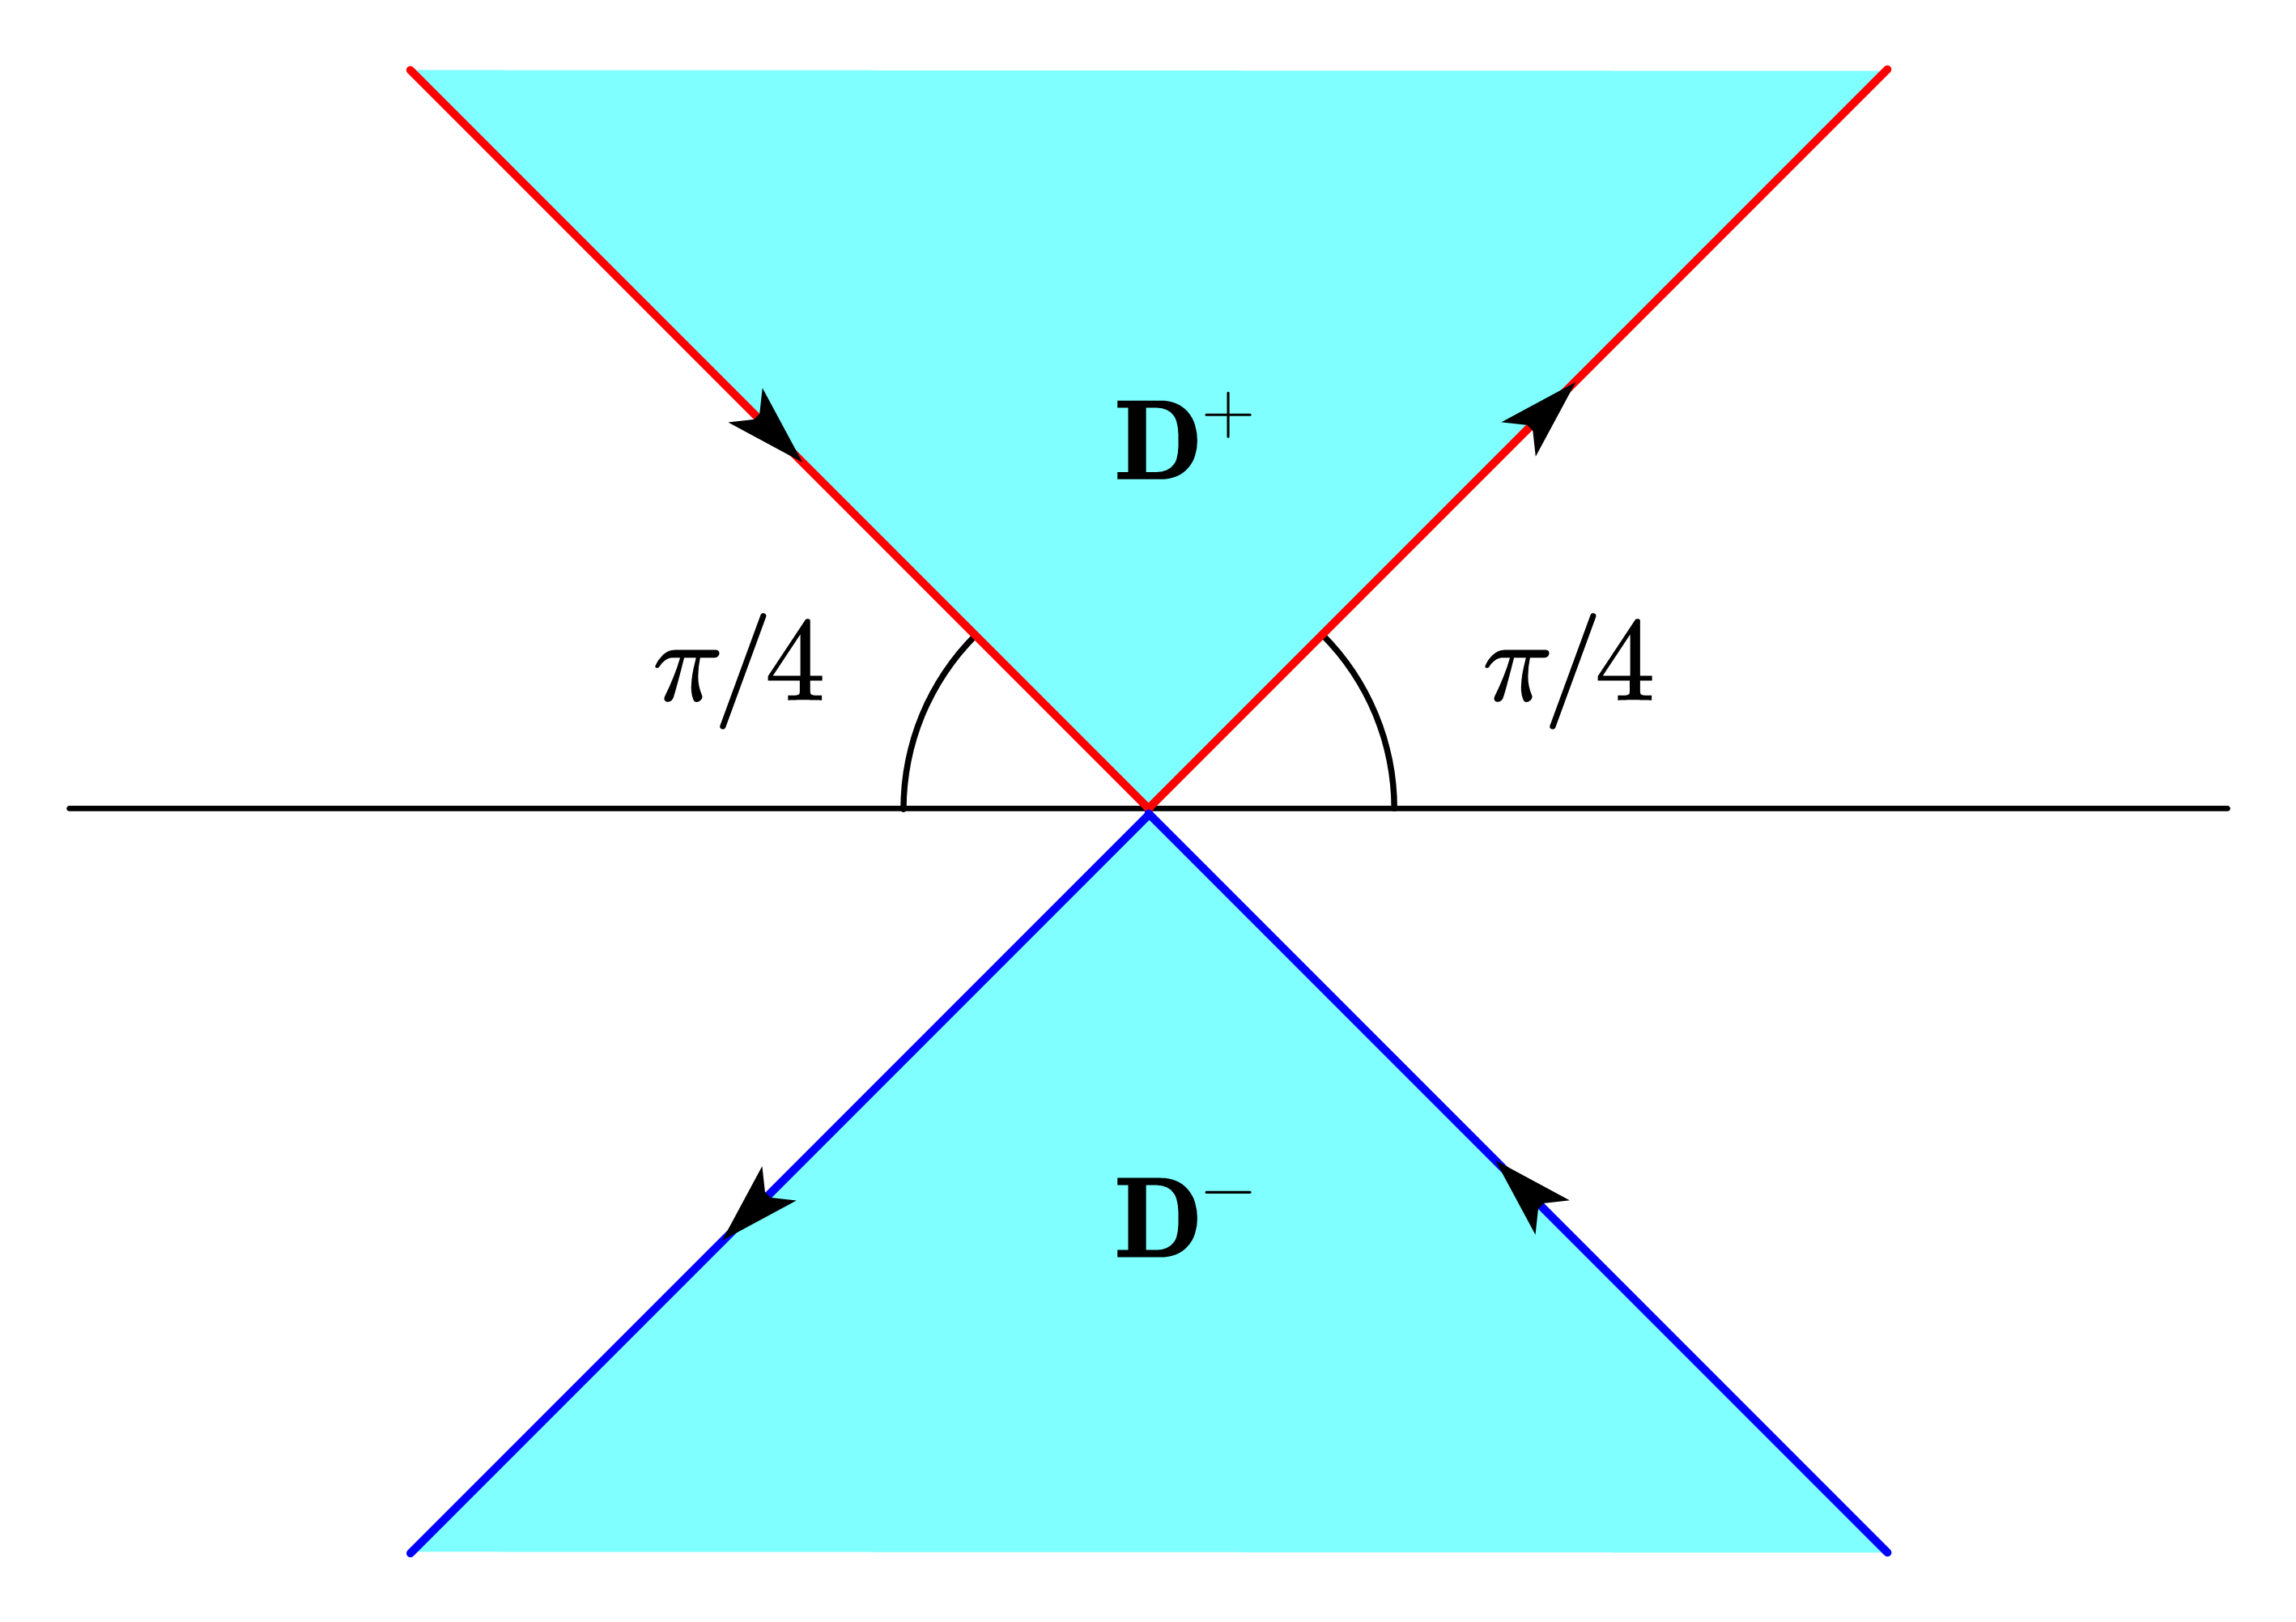
\includegraphics[width=0.60\textwidth]{D^+.pic.jpg}
    \caption{The regions $D^+$ and $D^-$ in the complex $\lambda$ plane, with $D=D^+\cup D^-$. The boundaries $\partial D^+$ and $\partial D^-$ are both equipped with counterclockwise orientation.}
    \label{4}
\end{figure}
Again, we apply the Inverse Fourier transform to Eq.\eqref{2.3}, shift the contour of integration by the Jordan's Lemma and Cauchy's theorem, we obtain
\begin{equation}\label{2.5}
    \begin{split}
        u(x,t)&=\dfrac{1}{2\pi}\int_{\mathbb{R}} e^{i\lambda x-\lambda^2 t} \hat{f}(\lambda)d\lambda-\dfrac{1}{2\pi}\int_{\partial D^+} e^{i\lambda x-\lambda^2 t}[\tilde{g}_1(\lambda^2,t)+i\lambda\tilde{g}_0(\lambda^2,t)]d\lambda\\
        &-\dfrac{1}{2\pi}\int_{\partial D^-} e^{-i\lambda(L-x)-\lambda^2 t}[\tilde{h}_1(\lambda^2,t)+i\lambda\tilde{h}_0(\lambda^2,t)]d\lambda,
    \end{split}
\end{equation}
where $\partial D^+$ and $\partial D^-$ are specified in figure(\ref{4}).

\subsection{Step 3\textemdash Eliminate the Unknowns}
Let's write the Global Relation Eq.\eqref{2.3} in terms of the knowns and unknowns,
\begin{equation}\label{2.6}
    e^{\lambda^2 t}\hat{u}(\lambda,t)=\Phi(\lambda,t)-\tilde{g}_1(\lambda^2,t)+e^{-i\lambda L}\tilde{h}_1(\lambda^2,t),
\end{equation}
where 
\begin{equation}
    \Phi(\lambda,t)=\hat{f}(\lambda)-i\lambda\tilde{g}_0(\lambda^2,t)+i\lambda e^{-i\lambda L}\tilde{h}_0(\lambda^2,t)
\end{equation}
is given. Similarly, let $\lambda\mapsto -\lambda$ in Eq.\eqref{2.6}, and recall $\tilde{g}_j$, $\tilde{h}_j$ $(j=0,1)$ are invariant under $\lambda\mapsto -\lambda$, we have that 
\begin{equation}\label{2.8}
    e^{\lambda^2 t}\hat{u}(-\lambda,t)=\Phi(-\lambda,t)-\tilde{g}_1(\lambda^2,t)+e^{i\lambda L}\tilde{h}_1(\lambda^2,t)
\end{equation}
Solving Eq.\eqref{2.6} and Eq.\eqref{2.8} for $\tilde{g}_1$ and $\tilde{h}_1$, we obtain
\begin{equation}
    \begin{split}
        \tilde{g}_1(\lambda^2,t)&=\dfrac{e^{i\lambda L}\Phi(\lambda,t)-e^{-i\lambda L}\Phi(-\lambda,t)}{e^{i\lambda L}-e^{-i\lambda L}}\\
        &+\dfrac{e^{\lambda^2 t}[e^{-i\lambda L}\hat{u}(-\lambda,t)-e^{i\lambda t}\hat{u}(\lambda,t)]}{e^{i\lambda L}-e^{-i\lambda L}}\\
        \tilde{h}_1(\lambda^2,t)&=\dfrac{\Phi(\lambda,t)-\Phi(-\lambda,t)+e^{\lambda^2 t}[\hat{u}(-\lambda,t)-\hat{u}(\lambda,t)]}{e^{i\lambda L}-e^{-i\lambda L}}.
    \end{split}
\end{equation}
We can then substitude $\tilde{g}_1$ and $\tilde{h}_1$ in Eq.\eqref{2.5}. We claim the terms involving $\hat{u}(\pm\lambda,t)$ yield a zero contribution. Consider the contributions
\begin{equation}\label{2.10}
    \begin{cases}
         &\dfrac{1}{2\pi}\displaystyle\int_{\partial D^+}\dfrac{e^{-i\lambda L}\hat{u}(-\lambda,t) -e^{i\lambda L}\hat{u}(\lambda,t)}{e^{i\lambda L}-e^{-i\lambda L}} e^{i\lambda x}d\lambda ;\\[5mm] 
         &\dfrac{1}{2\pi}\displaystyle\int_{\partial D^-}\dfrac{\hat{u}(-\lambda,t)-\hat{u}(\lambda,t)}{e^{i\lambda L}-e^{-i\lambda L}} e^{-i\lambda (L-x)}d\lambda .
    \end{cases}
\end{equation}
On $D^+$, $e^{-i\lambda L}$ grows exponentially, then 
\begin{equation}
    \lim\limits_{\lambda\to\infty} \dfrac{e^{-i\lambda L}\hat{u}(-\lambda,t) -e^{i\lambda L}\hat{u}(\lambda,t)}{e^{i\lambda L}-e^{-i\lambda L}}=-\hat{u}(-\lambda,t)+e^{i\lambda L}\int_{0}^{L} e^{i\lambda (L-x)}u(x,t)dx,
\end{equation}
which is bounded. On $D^-$, $e^{i\lambda L}$ grows exponentially, so 
\begin{equation}
    \lim\limits_{\lambda\to\infty} \dfrac{\hat{u}(-\lambda,t)-\hat{u}(\lambda,t)}{e^{i\lambda L}-e^{-i\lambda L}}=-e^{-i\lambda L}\hat{u}(\lambda,t)+\int_{0}^{L}e^{-i\lambda(L-x)}u(x,t)dx,
\end{equation}
which is also bounded. Moreover, observe that $\lambda=0$ is a removable singularity of both $\dfrac{e^{-i\lambda L}\hat{u}(-\lambda,t) -e^{i\lambda L}\hat{u}(\lambda,t)}{e^{i\lambda L}-e^{-i\lambda L}}$ and $\dfrac{\hat{u}(-\lambda,t)-\hat{u}(\lambda,t)}{e^{i\lambda L}-e^{-i\lambda L}}$. Because 
\begin{equation}
    \left.{e^{-i\lambda L}\hat{u}(-\lambda,t) -e^{i\lambda L}\hat{u}(\lambda,t)}\right\vert_{\lambda=0}=\left. \hat{u}(-\lambda,t)-\hat{u}(\lambda,t)\right\vert_{\lambda=0}=0,
\end{equation}
and $\lambda=0$ is a zero of order one of $e^{i\lambda L}-e^{-i\lambda L}$. Then, with the two functions holomorphic in the upper-half plane and the lower-half plane respectively, we apply the same arguments in subsection(\ref{SSec 1.3}) to verify that both terms in Eq.\eqref{2.10} vanish.
Therefore, Eq.\eqref{2.5} becomes 
\begin{equation}\label{2.14}
    \begin{split}
        u(x,t)&=\dfrac{1}{2\pi}\int_{\mathbb{R}} e^{i\lambda x-\lambda^2 t} \hat{f}(\lambda)d\lambda\\
        &-\dfrac{1}{2\pi}\int_{\partial D^+} e^{i\lambda x-\lambda^2t} \left(i\lambda\tilde{g}_0(\lambda^2,t)+\dfrac{e^{i\lambda L}\Phi(\lambda,t)-e^{-i\lambda L}\Phi(-\lambda,t)}{e^{i\lambda L}-e^{-i\lambda L}}\right)d\lambda\\
        &-\dfrac{1}{2\pi}\int_{\partial D^-} e^{-i\lambda(L-x)-\lambda^2 t}\left(i\lambda\tilde{h}_0(\lambda^2,t)+\dfrac{\Phi(\lambda,t)-\Phi(-\lambda,t)}{e^{i\lambda L}-e^{-i\lambda L}}\right)d\lambda.
    \end{split}
\end{equation}

\subsection{Improving the Solution to the Ehrenpreis's Form}
Eq.\eqref{2.1} is valid only when $t\in[0,T]$, let's introduce 
\begin{equation}
    \begin{split}
        \tilde{g}_0(\lambda)&=\int_{0}^{T} e^{\lambda \tau}g_0(\tau)d\tau,\quad \tilde{h}_0(\lambda)=\int_{0}^{T} e^{\lambda\tau} h_0(\tau)d\tau;\\
        \tilde{g}_1(\lambda)&=\int_{0}^{T} e^{\lambda \tau}g_1(\tau)d\tau,\quad \tilde{h}_1(\lambda)=\int_{0}^{T} e^{\lambda\tau} h_1(\tau)d\tau.
    \end{split}
\end{equation}
Then, Eq.\eqref{2.5} is equivalent to 
\begin{equation}\label{2.16}
    \begin{split}
    u(x,t)&=\dfrac{1}{2\pi}\int_{\mathbb{R}} e^{i\lambda x-\lambda^2 t} \hat{f}(\lambda)d\lambda-\dfrac{1}{2\pi}\int_{\partial D^+} e^{i\lambda x-\lambda^2 t}[\tilde{g}_1(\lambda^2)+i\lambda\tilde{g}_0(\lambda^2)]d\lambda\\
        &-\dfrac{1}{2\pi}\int_{\partial D^-} e^{-i\lambda(L-x)-\lambda^2 t}[\tilde{h}_1(\lambda^2)+i\lambda\tilde{h}_0(\lambda^2)]d\lambda.
    \end{split}
\end{equation}
In fact, Eq.\eqref{2.16} and Eq.\eqref{2.5} differ by 
\begin{equation}
    \begin{split}
        &\dfrac{1}{2\pi}\int_{\partial D^+} e^{i\lambda x}\left[ \int_{t}^{T} \left(e^{-\lambda^2(t-\tau)}g_1(\tau)+i\lambda e^{-\lambda^2(t-\tau)}g_0(\tau)\right)d\tau \right]d\lambda\\
        +&\dfrac{1}{2\pi}\int_{\partial D^+} e^{-i\lambda (L-x)}\left[ \int_{t}^{T} \left(e^{-\lambda^2(t-\tau)}h_1(\tau)+i\lambda e^{-\lambda^2(t-\tau)}h_0(\tau)\right)d\tau \right]d\lambda,
    \end{split}
\end{equation}
which vanishes according to the arguments in subsection(\ref{SSec 1.4}). Then, by an exact same approach in subsection(\ref{SSec 1.4}), we find that Eq.\eqref{2.14} is equivalent to 
\begin{equation}\label{2.18}
    \begin{split}
        u(x,t)&=\dfrac{1}{2\pi}\int_{\mathbb{R}} e^{i\lambda x-\lambda^2 t} \hat{f}(\lambda)d\lambda\\
        &-\dfrac{1}{2\pi}\int_{\partial D^+} e^{i\lambda x-\lambda^2t} \left(i\lambda\tilde{g}_0(\lambda^2)+\dfrac{e^{i\lambda L}\Phi(\lambda)-e^{-i\lambda L}\Phi(-\lambda)}{e^{i\lambda L}-e^{-i\lambda L}}\right)d\lambda\\
        &-\dfrac{1}{2\pi}\int_{\partial D^-} e^{-i\lambda(L-x)-\lambda^2 t}\left(i\lambda\tilde{h}_0(\lambda^2)+\dfrac{\Phi(\lambda)-\Phi(-\lambda)}{e^{i\lambda L}-e^{-i\lambda L}}\right)d\lambda,
    \end{split}
\end{equation}
where 
\begin{equation}
    \Phi(\lambda)=\hat{f}(\lambda)-i\lambda\tilde{g}_0(\lambda^2)+i\lambda e^{-i\lambda L}\tilde{h}_0(\lambda^2).
\end{equation}
Now, one can easily verify that Eq.\eqref{2.18} is the solution to Eq.\eqref{2.1}, because Eq.\eqref{2.18} is of the \href{https://w.wiki/9aTe}{Ehrenpreis's form} and one can pass the derivatives into the integrals using the \href{https://w.wiki/9asL}{Lebesgue dominated convergence theorem}.

\subsection{Rederiving the Series Solution}
It is possible to deform $\partial D^+$ and $\partial D^-$ back to the real axis and then apply the \href{https://w.wiki/9dCo}{Residue theorem} to recover the usual trigonometric solution. For simplicity, we assume homogeneous Dirichlet boundary conditions, that is, $g_0(t)=h_0(t)=0$, then the solution is now given by 
\begin{equation}\label{2.20}
    \begin{split}
        u(x,t)&=\dfrac{1}{2\pi}\int_{\mathbb{R}} e^{i\lambda x-\lambda^2t}\hat{f}(\lambda)d\lambda-\dfrac{1}{2\pi}\int_{\partial D^-} e^{-i\lambda(L-x)-\lambda^2 t}\left(\dfrac{\hat{f}(\lambda)-\hat{f}(-\lambda)}{e^{i\lambda L}-e^{-i\lambda L}}\right) d\lambda \\
        &-\dfrac{1}{2\pi}\int_{\partial D^+}e^{i\lambda x-\lambda^2 t}\left(\dfrac{e^{i\lambda L}\hat{f}(\lambda)-e^{-i\lambda L}\hat{f}(-\lambda)}{e^{i\lambda L}-e^{-i\lambda L}}\right) d\lambda.
    \end{split}
\end{equation}
To simplify the notation, let's define 
\begin{equation*}
    \begin{split}
    \phi^+(x,t,\lambda)&=e^{i\lambda x-\lambda^2 t}\left(\dfrac{e^{i\lambda L}\hat{f}(\lambda)-e^{-i\lambda L}\hat{f}(-\lambda)}{e^{i\lambda L}-e^{-i\lambda L}}\right),\quad \text{Im}(\lambda)\geqslant 0, \text{Re}(\lambda)\notin  \bigcup_{n\in\mathbb{Z}^*}\{\dfrac{n\pi}{L}\};\\
    \phi^-(x,t,\lambda)&=e^{-i\lambda(L-x)-\lambda^2 t}\left(\dfrac{\hat{f}(\lambda)-\hat{f}(-\lambda)}{e^{i\lambda L}-e^{-i\lambda L}}\right),\quad \text{Im}(\lambda)\leqslant 0, \text{Re}(\lambda)\notin  \bigcup_{n\in\mathbb{Z}^*}\{\dfrac{n\pi}{L}\}.
    \end{split}
\end{equation*}
\begin{figure}[h]
    \centering 
    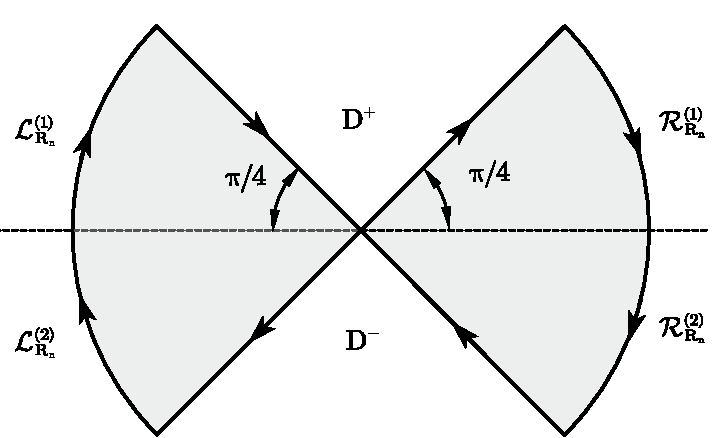
\includegraphics[width=0.60\textwidth]{Fokas 2.5.1.pdf}
    \caption{$\mathcal{R}^{(1)}_{R_n}=\{\lambda\in\mathbb{C}:\vert\lambda\vert=R_n=\frac{(2n+1)\pi}{2L},0\leqslant\arg{\lambda}\leqslant\pi/4\}$, $\mathcal{L}^{(1)}_{R_n}=\{\lambda\in\mathbb{C}:\vert\lambda\vert=R_n=\frac{(2n+1)\pi}{2L},3\pi/4\leqslant\arg{\lambda}\leqslant\pi\}$, $\mathcal{R}^{(2)}_{R_n}=\{\lambda\in\mathbb{C}:\vert\lambda\vert=R_n=\frac{(2n+1)\pi}{2L},7\pi/4\leqslant\arg{\lambda}\leqslant 2\pi\}$, $\mathcal{L}^{(2)}_{R_n}=\{\lambda\in\mathbb{C}:\vert\lambda\vert=R_n=\frac{(2n+1)\pi}{2L},\pi\leqslant\arg{\lambda}\leqslant 5\pi/4\}$, all equipped with clockwise orientation.}
    \label{5}
\end{figure}

Then, Jordan's lemma implies that 
\begin{equation}
    \begin{cases}
    &\lim\limits_{n\to\infty}\int_{\mathcal{L}^{(1)}_{R_n}} \phi^{+}(x,t,\lambda)d\lambda=\lim\limits_{n\to\infty}\int_{\mathcal{R}^{(1)}_{R_n}} \phi^{+}(x,t,\lambda)d\lambda=0,\\
    &\lim\limits_{n\to\infty}\int_{\mathcal{L}^{(2)}_{R_n}} \phi^{-}(x,t,\lambda)d\lambda=\lim\limits_{n\to\infty}\int_{\mathcal{R}^{(2)}_{R_n}} \phi^{-}(x,t,\lambda)d\lambda=0,
    \end{cases}
\end{equation}
where $\mathcal{L}^{(j)}_{R_n}$ and $\mathcal{R}^{(j)}_{R_n}$ are specified in figure(\ref{5}), for $j=1,2$.
\begin{figure}[h]
    \centering 
    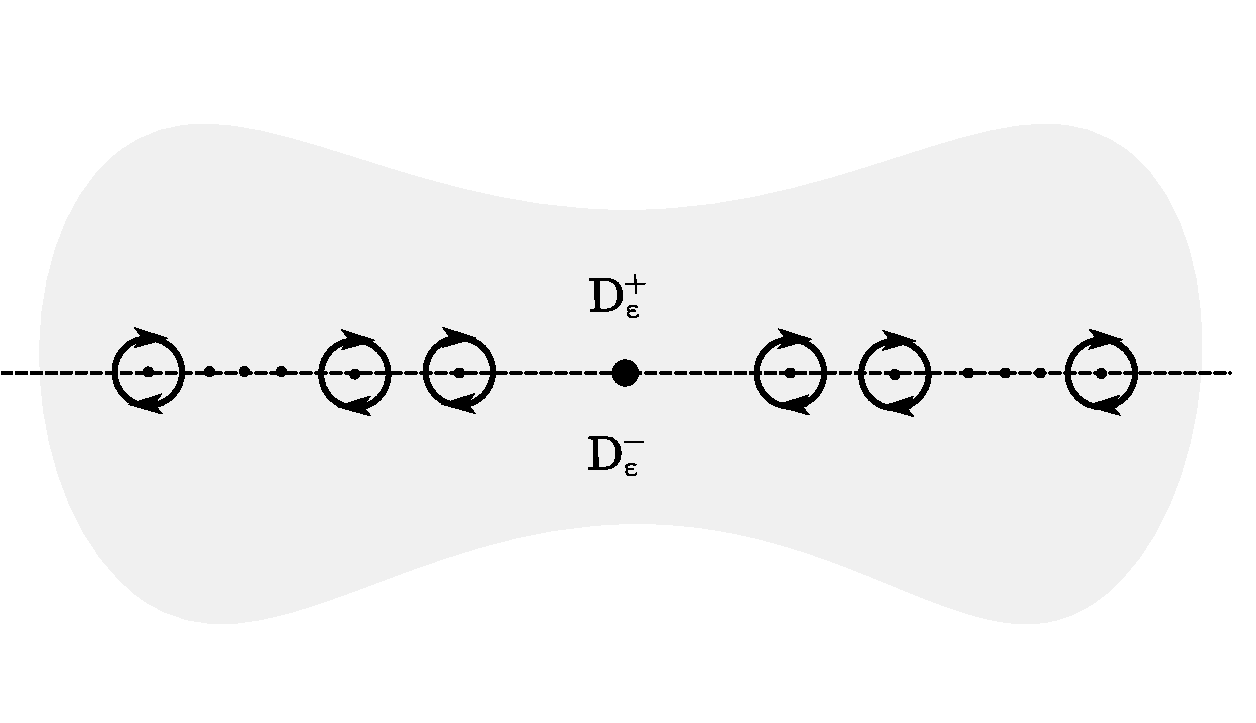
\includegraphics[width=0.60\textwidth]{Fokas 2.5.pdf}
    \caption{$D^+_{\varepsilon}=\{\lambda\in\mathbb{C}:\text{Im}(\lambda\geqslant 0)\}\setminus(\bigcup_{n\in\mathbb{Z}^*}D(n\pi/L,\varepsilon))$, with $\partial D^+_{\varepsilon}$ equipped with clockwise orientation; $D^-_{\varepsilon}=\{\lambda\in\mathbb{C}:\text{Im}(\lambda\leqslant 0)\}\setminus(\bigcup_{n\in\mathbb{Z}^*}D(n\pi/L,\varepsilon))$, with $\partial D^-_{\varepsilon}$ equipped with clockwise orientation, where $\varepsilon\ll\frac{\pi}{2L}$.}
    \label{6}
\end{figure}\\
With $D^{\pm}_{\varepsilon}$ specified in figure(\ref{6}), we can deform $\partial D^{\pm}$ to $\partial D^+_{\varepsilon}$ by Cauchy's theorem in Eq.\eqref{2.20} and write
\begin{equation*}
    \begin{split}
        u(x,t)&=\dfrac{1}{2\pi}\int_{\mathbb{R}} e^{i\lambda x-\lambda^2t}\hat{f}(\lambda)d\lambda-\dfrac{1}{2\pi}\int_{\partial D^-_{\varepsilon}} \phi^{-}(x,t,\lambda) d\lambda -\dfrac{1}{2\pi}\int_{\partial D^+_{\varepsilon}} \phi^{+}(x,t,\lambda) d\lambda.
    \end{split}
\end{equation*}
$\phi^{\pm}(x,t,\lambda)$ have only countably many simple poles along the real axis. But the symmetricity with respect to $\lambda$ in the definition for $\phi^{\pm}(x,t,\lambda)$ yields that 
\begin{equation}
    \begin{split}
    \int_{\partial D^+(n\pi/L,\varepsilon)}\phi^{+}(x,t,\lambda)d\lambda=-\pi i\cdot\text{Res}(\phi^{+},n\pi/L),\\
    \int_{\partial D^-(n\pi/L,\varepsilon)}\phi^{-}(x,t,\lambda)d\lambda=-\pi i\cdot\text{Res}(\phi^{-},n\pi/L),\\
    \end{split}
\end{equation}
where $\partial D^{+}(n\pi/L,\varepsilon)$ denotes the upper semi-circle centering at $n\pi/L$ with radius $\varepsilon$, $\partial D^{-}(n\pi/L,\varepsilon)$ denotes the lower semi-circle centering at $n\pi/L$ with radius $\varepsilon$, both equipped with clockwise orientation. Hence, we have that 
\begin{equation*}
    \begin{split}
        u(x,t)&=\dfrac{1}{2\pi}\int_{\mathbb{R}} e^{i\lambda x-\lambda^2t}\hat{f}(\lambda)d\lambda\\
        &-\dfrac{1}{2\pi}\left(\int_{\mathbb{R}\setminus(\cup_{n\in\mathbb{Z}^*}[n\pi/L-\varepsilon, n\pi/L+\varepsilon])}\phi^+(x,t,\lambda)d\lambda-\sum_{n\in\mathbb{Z}^*}\pi i\cdot \text{Res}(\phi^+,n\pi/L)\right)\\
        &+\dfrac{1}{2\pi}\left(\int_{\mathbb{R}\setminus(\cup_{n\in\mathbb{Z}^*}[n\pi/L-\varepsilon, n\pi/L+\varepsilon])}\phi^-(x,t,\lambda)d\lambda+\sum_{n\in\mathbb{Z}^*}\pi i\cdot \text{Res}(\phi^-,n\pi/L)\right)\\[1mm]
    \end{split}
\end{equation*}
\begin{equation*}
    \begin{split}
        &=\dfrac{1}{2\pi}\int_{\mathbb{R}} e^{i\lambda x-\lambda^2t}\hat{f}(\lambda)d\lambda-\dfrac{1}{2\pi}\int_{\mathbb{R}\setminus(\cup_{n\in\mathbb{Z}^*}[n\pi/L-\varepsilon, n\pi/L+\varepsilon])}\hat{f}(\lambda)d\lambda\\
        &+\dfrac{i}{2}\sum_{n\in\mathbb{Z}^*}\{\text{Res}(\phi^+,n\pi/L)+\text{Res}(\phi^-,n\pi/L)\}.
    \end{split}
\end{equation*}
By passing $\varepsilon\to 0$, we find that the first two integrals cancel each other, so 
\begin{equation}\label{2.23}
    \begin{split}
        u(x,t)&=\dfrac{i}{2}\sum_{z\in\mathbb{Z}^*}\{\text{Res}(\phi^+,n\pi/L)+\text{Res}(\phi^-,n\pi/L)\}\\
        &=\dfrac{i}{2}\sum_{z\in\mathbb{Z}^*}\left(\lim\limits_{\lambda\to n\pi/L}(\lambda-n\pi/L)[\phi^{+}(x,t,L)+\phi^{-}(x,t,L)]\right)\\
        &=-\dfrac{i}{2}\sum_{z\in\mathbb{Z}^*} e^{i\lambda_n x-\lambda^2_n t}\left(\dfrac{2}{L}\int_{0}^{L}\sin(\lambda_n x)f(x)dx\right)\\
        &=\sum_{n=1}^{\infty} \left(\dfrac{2}{L}\int_{0}^{L}\sin(\lambda_n x)f(x)dx\right)e^{-\lambda^2_n t}\sin(\lambda_n x),
    \end{split}
\end{equation}
where $\lambda_n=n\pi/L$, the last equality is due to the property that 
\begin{equation}
    f_n=\left(\dfrac{2}{L}\int_{0}^{L}\sin(\lambda_n x)f(x)dx\right)=-f_{-n}.
\end{equation}
Therefore, we obtain the classical sine series representation of the solution to Eq.\eqref{2.1}, which is given by Eq.\eqref{2.23}.




\newpage
\bibliographystyle{unsrt} % Specify the bibliography style
\bibliography{references} % Include the bibliography file




































\end{document}
